\documentclass[supercite]{Experimental_Report}

\title{数据结构实验}
\author{刘文博}
%\coauthor{张三、李四}
\school{计算机科学与技术学院}
\classnum{计算机本硕博}
\stunum{U202115666}
%\costunum{}
\instructor{向文} % 该系列实验报告模板有华科大计院教师陈加忠制作
\date{2022年6月11日}

\usepackage{algorithm, multirow}
\usepackage{algpseudocode}
\usepackage{amsmath}
\usepackage{amsthm}
\usepackage{framed}
\usepackage{mathtools}
\usepackage{subcaption}
\usepackage{xltxtra} %提供了针对XeTeX的改进并且加入了XeTeX的LOGO, 自动调用xunicode宏包(提供Unicode字符宏)
\usepackage{bm}
\usepackage{tikz}
\usepackage{tikzscale}
\usepackage{pgfplots}
\usepackage{listings}
%\usepackage{enumerate}

\pgfplotsset{compat=1.16}

\newcommand{\cfig}[3]{
	\begin{figure}[htb]
		\centering
		\includegraphics[width=#2\textwidth]{images/#1.png}
		\caption{#3}
		\label{fig:#1}
	\end{figure}
}

\newcommand{\sfig}[3]{
	\begin{subfigure}[b]{#2\textwidth}
		\includegraphics[width=\textwidth]{images/#1.png}
		\caption{#3}
		\label{fig:#1}
	\end{subfigure}
}

\newcommand{\xfig}[3]{
	\begin{figure}[htb]
		\centering
		#3
		\caption{#2}
		\label{fig:#1}
	\end{figure}
}

\newcommand{\rfig}[1]{\autoref{fig:#1}}
\newcommand{\ralg}[1]{\autoref{alg:#1}}
\newcommand{\rthm}[1]{\autoref{thm:#1}}
\newcommand{\rlem}[1]{\autoref{lem:#1}}
\newcommand{\reqn}[1]{\autoref{eqn:#1}}
\newcommand{\rtbl}[1]{\autoref{tbl:#1}}

\algnewcommand\Null{\textsc{null }}
\algnewcommand\algorithmicinput{\textbf{Input:}}
\algnewcommand\Input{\item[\algorithmicinput]}
\algnewcommand\algorithmicoutput{\textbf{Output:}}
\algnewcommand\Output{\item[\algorithmicoutput]}
\algnewcommand\algorithmicbreak{\textbf{break}}
\algnewcommand\Break{\algorithmicbreak}
\algnewcommand\algorithmiccontinue{\textbf{continue}}
\algnewcommand\Continue{\algorithmiccontinue}
\algnewcommand{\LeftCom}[1]{\State $\triangleright$ #1}

\newtheorem{thm}{定理}[section]
\newtheorem{lem}{引理}[section]

\colorlet{shadecolor}{black!15}

\theoremstyle{definition}
\newtheorem{alg}{算法}[section]

\def\thmautorefname~#1\null{定理~#1~\null}
\def\lemautorefname~#1\null{引理~#1~\null}
\def\algautorefname~#1\null{算法~#1~\null}
\lstset{
	basicstyle=\tt,
	keywordstyle=\bfseries\color{purple},
	identifierstyle=\color{brown!80!black},
	commentstyle=\color{gray}
	breaklines=true,	
	columns=flexible,
	showspaces=false,
	showtabs=false,
	showstringspaces=true,
	frame=single,
}
\begin{document}
		
\maketitle

\clearpage

\pagenumbering{Roman}

\tableofcontents[level=2]

\clearpage

\pagenumbering{arabic}
		
		
\section{基于链式存储结构的线性表实现}

\subsection{问题描述}
\noindent 实验要求:
\begin{enumerate}
	\item 实现对链表的基本操作;
	\item 选择性实践对链表的进阶操作;
	\item 设计演示系统。
\end{enumerate}
通过实验达到:
\begin{enumerate}
	\item 加深对线性表的概念、基本运算的理解;
	\item 熟练掌握线性表的逻辑结构与物理结构的关系;
	\item 物理结构采用单链表,熟练掌握线性表的基本运算的实现。
\end{enumerate}
分析:需要了解链表的结构,同时演示系统要清晰明了。

		\subsection{系统设计}

\subsubsection{演示系统菜单的组织架构}
\cfig{2.1}{0.6}{演示系统模块结构图}
\newpage
\quad 演示系统分为基本操作和进阶操作两部分,以一个菜单为主界面,以序号1至12表示创建,销毁,清空,插入,删除,求表长等基本操作,以序号13至17表示保存为文件,加载文件,翻转链表,对链表排序等进阶操作,以序号0表示退出演示系统,根据序号调用函数执行操作。
\cfig{2.2}{0.6}{演示系统流程图}
\subsubsection{ADT数据结构设计}
\noindent 对链表数据类型的定义如下\par
\begin{lstlisting}[language=C] 
	typedef int status;
	typedef int ElemType;
	typedef struct LNode{单链表(链式结构)结点的定义
		ElemType data;
		struct LNode* next;
	}LNode, *LinkList;
\end{lstlisting}
对一些常量的定义如下
\begin{lstlisting}[language=C] 
	#define LIST_INIT_SIZE 100
	#define LISTINCREMENT  10
	#define TRUE 1
	#define FALSE 0
	#define OK 1
	#define ERROR 0
	#define INFEASIBLE -1
	#define OVERFLOW -2
\end{lstlisting}

\subsubsection{初始化表}
输入:顺序表(未知状态)

输出:函数执行状态

算法的思想描述:为L结点分配存储空间,将L->next结点置空

算法处理步骤:
\begin{enumerate}
	\renewcommand{\labelenumi}{\theenumi)}
	\item 如果顺序表L不存在,则为L分配存储空间。
	\item 如果分配成功,将L->next置空返回状态OK。
	\item 如果分配失败,返回状态 OVERFLOW 并推出该程序块。
	\item 如果顺序表存在,返回状态 INFEASIBLE 以指出无法创建。
\end{enumerate}

时间复杂度:O(1)

空间复杂度:O(1)

\cfig{1.2.3}{0.8}{初始化表流程图}
\subsubsection{销毁表}
输入:顺序表(未知状态)

输出:函数执行状态

算法的思想描述:若 L 为 NULL,返回 INFEASIBLE。用 while 循环依次释放所有节点的储存空间,再将 L 置为 NULL。

\begin{lstlisting}[language=C] 
	status DestroyList(LinkList &L)
	{
		if(!L) return INFEASIBLE;
		LinkList p;
		while(L)
		{
			p=L;
			L=L->next;
			free(p);
		}
		return OK;
	}
\end{lstlisting}

时间复杂度:O(n)

空间复杂度:O(1)
\subsubsection{清空表}
输入:顺序表(未知状态)

输出:函数执行状态

算法的思想描述:若 L 为 NULL,返回 INFEASIBLE。\\否则用while循环释放除头节点以外的所有节点的储存空间,再将 L->next 置为 NULL。

\begin{lstlisting}[language=C] 
	status ClearList(LinkList &L)
	{
		if(!L) return INFEASIBLE;
		LinkList p;
		while(L->next)
		{
			p=L->next;
			L->next=p->next;
			free(p);
		}
		return OK;
	}
\end{lstlisting}

时间复杂度:O(n)

空间复杂度:O(1)
\subsubsection{表判空}
输入:顺序表(未知状态)

输出:函数执行状态

算法的思想描述:若 L 为 NULL,返回 INFEASIBLE。否则判断 L->next 是否为 NULL,若为 NULL,则链表为空,否则链表不为空。
\begin{lstlisting}[language=C] 
	status ListEmpty(LinkList L)
	{
		if(!L) return INFEASIBLE;
		if(!L->next) return TRUE;
		else return FALSE;
		
	}
\end{lstlisting}

时间复杂度:O(1)

空间复杂度:O(1)
\subsubsection{求表长}

输入:顺序表L

输出:顺序表的长度

算法思想描述:遍历整个顺序表

算法处理步骤:
\begin{enumerate}
	\renewcommand{\labelenumi}{\theenumi)}
	\item 如果顺序表L不存在,则输出INFEASIBLE。
	\item 如果L存在,从头开始遍历。
	\item 若不为空则移动指针到下一个结点,长度加1。
	\item 返回长度的值。
\end{enumerate}

时间复杂度:O(n)

空间复杂度:O(1)
\cfig{1.2.4}{0.8}{求表长流程图}
\subsubsection{获取元素}
输入:顺序表(未知状态)

输出:L中第i个数据元素的值e

算法的思想描述:若 L 为 NULL,返回 INFEASIBLE。若 i 小于 1 或大于链表的长度,则该序号非法,返回 ERROR。否则遍历至第 i 个元素,返回其数据域的值。	
\begin{lstlisting}[language=C] 
	status GetElem(LinkList L,int i,ElemType &e)
	{
		if(!L) return INFEASIBLE;
		if(i<=0) return ERROR;
		LinkList p=L;
		for(int j=0;j<i;j++)
		{
			p=p->next;
			if(!p) return ERROR;
		}
		e=(*p).data;
		return OK;
	}
\end{lstlisting}

时间复杂度:O(n)

空间复杂度:O(1)
\subsubsection{定位元素}
输入:顺序表(未知状态)

输出:L中第1个与e相等的元素的序号,若这样的数据元素不存在,则值为 0

算法的思想描述:若 L 为 NULL,返回 INFEASIBLE。否则声明 i=0,遍历链表查找是
否有值与 e 相同的元素,每进入下一个节点时 i 自增,若找到相应元素则返回 i,
否则返回 ERROR。
\begin{lstlisting}[language=C] 
	status LocateElem(LinkList L,ElemType e)
	{
		if(!L) return INFEASIBLE;
		LinkList p=L->next;
		int ans=1;
		while(p)
		{  
			if((*p).data==e) return ans;
			ans++;
			p=p->next;
		}
		return ERROR;
	}
\end{lstlisting}

时间复杂度:O(n)

空间复杂度:O(1)
\newpage
\subsubsection{获得前驱}

输入:顺序表L,元素e,引用参数pre。

输出:函数的执行状态.

算法思想的描述:遍历顺序表.

算法处理步骤:
\begin{enumerate}
	\renewcommand{\labelenumi}{\theenumi)}
	\item 如果顺序表L不存在,则输出INFEASIBLE。
	\item 如果L存在,从头开始遍历。
	\item 若当前节点的后继值为e,则将当前节点的值赋给pre,输出OK。
	\item 若为找到,则返回INFEASIBLE.
\end{enumerate}

时间复杂度:O(n)

空间复杂度:O(1)
\cfig{1.2.5}{0.8}{求前驱流程图}
\subsubsection{求后继}
输入:顺序表(未知状态)

输出:函数执行状态

算法的思想描述:若 L 为 NULL,返回 INFEASIBLE。否则链表查找值等于 e 的元素,
若找到则将该节点后继节点的数据域赋值给 next,否则返回 ERROR。	
\begin{lstlisting}[language=C] 
	status NextElem(LinkList L,ElemType e,ElemType &next)
	{
		if(!L) return INFEASIBLE;
		LinkList p=L->next;
		if(!p) return ERROR;
		LinkList q=p->next;
		while(q)
		{  
			if((*p).data==e) 
			{
				next=(*q).data;
				return OK;
			}
			p=p->next;
			q=q->next;
		}
		return ERROR;
	}
\end{lstlisting}

时间复杂度:O(n)

空间复杂度:O(1)
\subsubsection{插入元素}

输入:顺序表L,插入位置I,插入元素e。

输出:函数的执行状态。

算法的思想描述:查找元素和移动之后的结点.

算法处理步骤:
\begin{enumerate}
	\renewcommand{\labelenumi}{\theenumi)}
	\item 如果顺序表L不存在,则输出INFEASIBLE。
	\item 如果L存在,判断i值是否符合要求,不符合则返回ERROR。
	\item 如果I值合法,增加一个新的结点用于存储插入元素。
	\item 将插入位置前的结点指向新插入的节点,将新节点指向插入位置后一个节点.
	\item 返回OK。
\end{enumerate}

时间复杂度:O(n)

空间复杂度:O(1)
\cfig{1.2.6}{0.8}{插入元素流程图}
\subsubsection{删除元素}
输入:顺序表(未知状态)

输出:函数执行状态

算法的思想描述:若 L 为 NULL,返回 INFEASIBLE。若 i 小于 1 或大于链表长度则返回 ERROR。否则遍历至链表第 i-1 个元素,将其指针域置为其后继的后继,数据赋给 e,最后释放其后继节点。
\begin{lstlisting}[language=C] 
	status ListDelete(LinkList &L,int i,ElemType &e)
	{
		if(!L) return INFEASIBLE;
		LinkList p=L,q;
		int ans=1;
		if(L->next) q=L->next;
		if(i<=0) return ERROR;
		for(ans;ans<i;ans++)
		{  
			p=p->next;
			if(q->next) q=q->next;
			else return ERROR;
		}
		p->next=q->next;
		e=(*q).data;
		free(q);
		return OK;
	}
\end{lstlisting}

时间复杂度:O(n)

空间复杂度:O(1)
\subsubsection{遍历链表}
输入:顺序表L.

输出:函数的执行状态

算法思想描述:遍历链表并输出每一个元素的值.
\begin{enumerate}
	\renewcommand{\labelenumi}{\theenumi)}
	\item 如果顺序表L不存在,则输出INFEASIBLE。
	\item 如果L存在,从头开始遍历并输出。
	\item 返回OK。
\end{enumerate}

时间的复杂度:O(n).

空间的复杂度:O(1).
\cfig{1.2.7}{0.8}{遍历链表流程图}
\newpage 
\subsubsection{链表的翻转} 

输入:顺序表L

输出:链表翻转

算法的思想描述:利用栈这一数据结构,遍历让所有元素入栈再出栈,即可得到翻转的结果.

算法处理的步骤:
\begin{enumerate}
	\renewcommand{\labelenumi}{\theenumi)}
	\item 如果L不存在则为空表,输出ERROR并退出.
	\item 建立一个新的节点,遍历所有节点以栈的形式存储
	\item 改变头节点为栈的头节点
\end{enumerate}

时间复杂度:O(n)

空间复杂度:O(n)
\cfig{1.2.8}{0.5}{翻转链表流程图}
\subsubsection{删除链表的倒数第 n 个节点}
输入:顺序表(未知状态)

输出:函数执行状态

算法的思想描述:如果 L 为 NULL,返回 INFEASIBLE。否则调用求表长函数和删除节点函数,通过数学运算来实现倒数第 n 个元素的删除。	
\begin{lstlisting}[language=C] 
	status RemoveNthFromEnd(LinkList L, int n, ElemType& e)
	{
		if(!L) return INFEASIBLE;
		else
		{
			int k,j; 
			if(L->next==NULL) return ERROR;
			k = ListLength(L);
			j = k - n + 1;
			ListDelete(L, j, e);
			return OK;
		}
	}
\end{lstlisting}

时间复杂度:O(n)

空间复杂度:O(1)
\subsubsection{读入文件}
输入:顺序表(未知状态)

输出:函数执行状态

算法的思想描述:若 L 为 NULL,返回 INFEASIBLE。打开文件,从文件中每读入一个数据创建一个节点,并置为上一个结点的后继,直到读取完所有数据,关闭文件。
\begin{lstlisting}[language=C] 
	status LoadList(LinkList &L,char FileName[])
	{
		if(L) return INFEASIBLE;
		L=(LNode*)malloc(sizeof(LNode));
		FILE *fp=fopen(FileName,"r");
		if(!fp) return ERROR;
		ElemType e;
		LinkList p=L;
		while((fscanf(fp,"%d",&e))==1)
		{
			p->next=(LNode*)malloc(sizeof(LNode));
			p=p->next;
			(*p).data=e;
		}
		p->next=NULL;
		fclose(fp);
		return OK;
	}
\end{lstlisting}

时间复杂度:O(n)

空间复杂度:O(1)
\subsubsection{写入文件}
输入:顺序表(未知状态)

输出:函数执行状态

算法的思想描述:若 L 为 NULL,返回 INFEASIBLE。打开文件,遍历链表将所有元素的数据域写入文件,关闭文件。
\begin{lstlisting}[language=C] 
	status SaveList(LinkList L,char FileName[])
	{
		if(!L)
		{
			return INFEASIBLE;
		}
		else
		{
			LinkList p=L;
			FILE *fp=fopen(FileName,"w+");
			if(!fp) return ERROR;
			while(p->next)
			{
				p=p->next;
				fprintf(fp,"%d ",(*p).data);
			}
			fclose(fp);
			return OK;
		}
	}
\end{lstlisting}

时间复杂度:O(n)

空间复杂度:O(1)

\subsubsection{链表排序}
输入:顺序表(未知状态)

输出:函数执行状态

算法的思想描述:采用插入排序的方法对链表内元素进行大小排序。	
\begin{lstlisting}[language=C] 
	status SortList(LinkList L)
{
	LinkList p, q;
	if(!L) return INFEASIBLE;
	else
	{
	if(L->next==NULL) return ERROR;
int n = ListLength(L);
int i, j, temp;
for(i = 0,p = L -> next; i < n-1; i++,p = p -> next)
{
	for(j = i + 1,q = p -> next; j < n; j++,q = q -> next)
{
	if(p -> data > q -> data)
	{
		temp = p -> data;
		p -> data = q -> data;
		q -> data = temp;
	}
}
}		return OK;
	}	
}
\end{lstlisting}
时间复杂度:O(n)

空间复杂度:O(1)
\subsection{系统实现}
\subsubsection{程序开发环境与语言}
PC操作系统为windows操作系统使用语言为C++。
\subsubsection{代码的组织结构}
演示系统以一个菜单作为交互界面,用户通过输入命令对应的编号来调用相应的函数来实现创建表,销毁表,清空表,插入元素,删除元素,求表长,判空表,求前驱,求后继,遍历链表等基本操作,以及保存为文件,加载文件,翻转链表,对链表排序等进阶操作。


程序主函数为一个switch结构,根据输入的数字,执行不同的语句,进而调用不同的函数,宏定义函数返回值ERROR为0,INFEASIBLE为-1,OVERFLOW为-2,OK为1.
交互界面如下图
\cfig{1.3.1}{0.8}{交互界面示例}
\newpage
\subsection{系统测试}
程序开发及实现环境:Win11 下使用 Dev C++ 进行编译和调试,开发语言为 C 语言。

\quad 表\ref{table3.1}为正常样例测试的输入,预期结果与实际输出。
\begin{table}[p]
	\centering
	\caption{正常样例测试}
	\label{table3.1}
	\scalebox{0.7}{
		\begin{tabular}{|l|l|l|l|}
			\hline
			函数       & 输入                                                      & 实际输出                                                       &预期结果        \\ \hline
			初始化表      & 1                                                          & \begin{minipage}[b]{0.3\columnwidth} \centering \raisebox{-.5\height}{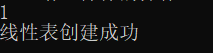
\includegraphics[width=\linewidth]{images/1.4.1.png}} \end{minipage}              &线性表创建成功    \\ \hline
			销毁表      & 2                                                          & \begin{minipage}[b]{0.3\columnwidth} \centering \raisebox{-.5\height}{
\includegraphics[width=\linewidth]{images/1.4.2.png}} \end{minipage}              &线性表销毁成功    \\ \hline
			销毁表      & 2                                                          & \begin{minipage}[b]{0.3\columnwidth} \centering \raisebox{-.5\height}{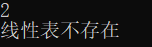
\includegraphics[width=\linewidth]{images/1.4.3.png}} \end{minipage}              &线性表不存在    \\ \hline
			初始化表      & 1                                                          & \begin{minipage}[b]{0.3\columnwidth} \centering \raisebox{-.5\height}{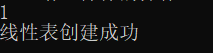
\includegraphics[width=\linewidth]{images/1.4.4.png}} \end{minipage}              &线性表创建成功    \\ \hline
			线性表判空      & 4                                                          & \begin{minipage}[b]{0.3\columnwidth} \centering \raisebox{-.5\height}{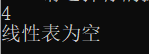
\includegraphics[width=\linewidth]{images/1.4.5.png}} \end{minipage}              &线性表为空    \\ \hline
			插入元素     & 10 1 1                                                          & \begin{minipage}[b]{0.3\columnwidth} \centering \raisebox{-.5\height}{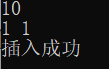
\includegraphics[width=\linewidth]{images/1.4.6.png}} \end{minipage}              &插入成功    \\ \hline
			插入元素      & 10 2 5                                                          & \begin{minipage}[b]{0.3\columnwidth} \centering \raisebox{-.5\height}{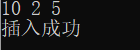
\includegraphics[width=\linewidth]{images/1.4.7.png}} \end{minipage}              &插入成功    \\ \hline
			插入元素     & 10 3 7                                                          & \begin{minipage}[b]{0.3\columnwidth} \centering \raisebox{-.5\height}{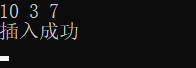
\includegraphics[width=\linewidth]{images/1.4.8.png}} \end{minipage}              &插入成功   \\ \hline
			求表长      & 5                                                          & \begin{minipage}[b]{0.3\columnwidth} \centering \raisebox{-.5\height}{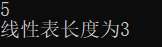
\includegraphics[width=\linewidth]{images/1.4.9.png}} \end{minipage}              &线性表长度为 3   \\ \hline
			获取元素      & 6 2                                                          & \begin{minipage}[b]{0.3\columnwidth} \centering \raisebox{-.5\height}{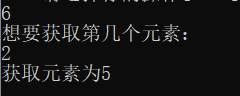
\includegraphics[width=\linewidth]{images/1.4.10.png}} \end{minipage}              &获取元素为 5    \\ \hline
			查找元素      & 7 7                                                          & \begin{minipage}[b]{0.3\columnwidth} \centering \raisebox{-.5\height}{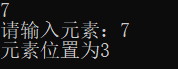
\includegraphics[width=\linewidth]{images/1.4.11.png}} \end{minipage}              &元素位置为 3    \\ \hline
			查找前驱      & 8 5                                                          & \begin{minipage}[b]{0.3\columnwidth} \centering \raisebox{-.5\height}{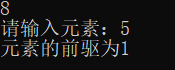
\includegraphics[width=\linewidth]{images/1.4.12.png}} \end{minipage}              &元素的前驱为 1  \\ \hline
			查找后继      & 9 5                                                          & \begin{minipage}[b]{0.3\columnwidth} \centering \raisebox{-.5\height}{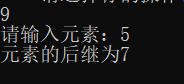
\includegraphics[width=\linewidth]{images/1.4.13.png}} \end{minipage}              &元素的后继为 7    \\ \hline
			遍历      & 12                                                          & \begin{minipage}[b]{0.3\columnwidth} \centering \raisebox{-.5\height}{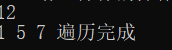
\includegraphics[width=\linewidth]{images/1.4.14.png}} \end{minipage}              &1 5 7 遍历完成    \\ \hline
			删除元素      & 11 2                                                          & \begin{minipage}[b]{0.3\columnwidth} \centering \raisebox{-.5\height}{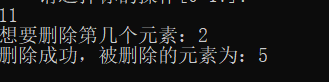
\includegraphics[width=\linewidth]{images/1.4.15.png}} \end{minipage}              &删除元素5   \\ \hline
			保存文件      & 13 123                                                          & \begin{minipage}[b]{0.3\columnwidth} \centering \raisebox{-.5\height}{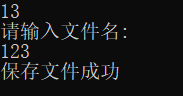
\includegraphics[width=\linewidth]{images/1.4.16.png}} \end{minipage}              &保存文件成功     \\ \hline
			销毁表      & 2                                                          & \begin{minipage}[b]{0.3\columnwidth} \centering \raisebox{-.5\height}{
\includegraphics[width=\linewidth]{images/1.4.17.png}} \end{minipage}              &线性表销毁成功    \\ \hline
			读取文件      & 17 F”:/shiyan                                                         & \begin{minipage}[b]{0.3\columnwidth} \centering \raisebox{-.5\height}{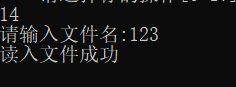
\includegraphics[width=\linewidth]{images/1.4.18.png}} \end{minipage}              &读入文件成功    \\ \hline
			遍历链表      & 12                                                          & \begin{minipage}[b]{0.3\columnwidth} \centering \raisebox{-.5\height}{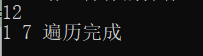
\includegraphics[width=\linewidth]{images/1.4.19.png}} \end{minipage}              &1 7 遍历完成    \\ \hline
		\end{tabular}
	}
\end{table}
\quad 表\ref{table3.2}为异常样例的输入,实际输出和对输出结果的分析\\
\begin{table}[b]
	\centering
	\caption{异常样例测试}
	\label{table3.2}
	\scalebox{0.7}{
		\begin{tabular}{|l|l|l|l|}
			\hline
			异常样例    & 输入            & 实际输出                                                                 & 结果分析       \\ \hline
			销毁表      & 2                                                          & \begin{minipage}[b]{0.3\columnwidth} \centering \raisebox{-.5\height}{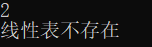
\includegraphics[width=\linewidth]{images/1.4.20.png}} \end{minipage}              &线性表不存在    \\ \hline
			清空表      & 3                                                          & \begin{minipage}[b]{0.3\columnwidth} \centering \raisebox{-.5\height}{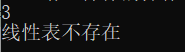
\includegraphics[width=\linewidth]{images/1.4.21.png}} \end{minipage}              &线性表不存在    \\ \hline
			获取元素 & 6                                                             & \begin{minipage}[b]{0.3\columnwidth} \centering 
				\raisebox{-.5\height}{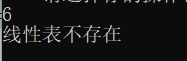
\includegraphics[width=\linewidth]{images/1.4.22.png}} \end{minipage}              &线性表不存在   \\ \hline
			查找后继 & 9 3                                                           & \begin{minipage}[b]{0.3\columnwidth} \centering \raisebox{-.5\height}{
\includegraphics[width=\linewidth]{images/1.4.23.png}} \end{minipage}                     &元素3没有后继元素  \\ \hline          
			插入元素 & 10 5 5                                                        & \begin{minipage}[b]{0.3\columnwidth} \centering \raisebox{-.5\height}{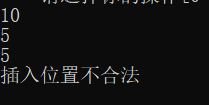
\includegraphics[width=\linewidth]{images/1.4.24.png}} \end{minipage}                     &插入元素的位置不合法  \\ \hline    
			读取文件 & 17                                                            & \begin{minipage}[b]{0.3\columnwidth} \centering \raisebox{-.5\height}{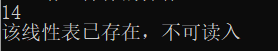
\includegraphics[width=\linewidth]{images/1.4.25.png}} \end{minipage}                    &线性表已存在   \\ \hline
		\end{tabular}
	}
\end{table}
\quad 通过异常用例可以看出,演示系统对表不存在时对除创建表以外的操作和对查找表中没有的元素的前驱、后继或对无后继、无前驱的元素要求获取后继、前驱的操作,以及在表存在时要求读取文件的操作的判定能力,可见演示系统能够识别异常样例。
\clearpage

\subsection{实验小结}
本次实验让我对基于链式存储结构的线性表的了解更进了一步。\par
演示系统的搭建,让我体会到了主函数和子函数的关系,以及如何搭建一个可以调用不同模块的系统。\par
在编写插入和删除乃至翻转链表的函数时,如何有条理地更改指针的指向是一大难点,比如在插入新结点时,必须先让新节点的指针域指向p指针所指元素的next,然后才能让p指向新节点,反之则会大错特错。经过这次实验,我明白了赋值顺序对程序的巨大影响。\par
总的来说,本次数据结构实验提高了我的编程能力,让我对系统整体设计有了更深的认识。
\clearpage

\section{基于邻接表的图实现}
\subsection{问题描述}
\noindent 实验要求:
\begin{enumerate}
	\item 实现对图的基本操作;
	\item 选择性实践对图的进阶操作;
	\item 设计演示系统。
\end{enumerate}
通过实验达到:
\begin{enumerate}
	\item 加深对图的概念、基本运算的理解;	
	\item 熟练掌握图的逻辑结构与物理结构的关系;
	\item 以邻接表作为物理结构,熟练掌握图基本运算的实现。
\end{enumerate}
分析:需要了解图的结构,同时演示系统要清晰明了。

\subsection{系统设计}

\subsubsection{演示系统菜单的组织架构}
\cfig{2.3}{0.6}{演示系统模块结构图}
\newpage
\quad 演示系统分为基本操作和进阶操作两部分,以一个菜单为主界面,以序号1至12表示创建,销毁,清空,插入,删除,遍历等基本操作,以序号13至17表示保存为文件,求最短通路,求距某顶点距离小于d的顶点,对顶点进行修改等进阶操作,以序号0表示退出演示系统,根据序号调用函数执行操作。
\cfig{2.4}{0.8}{演示系统流程图}
\subsubsection{ADT数据结构设计}
\noindent 对图数据类型的定义如下\par
\begin{lstlisting}[language=C] 
	typedef struct 
	{
		KeyType  key;
		char others[20];
	} VertexType; 顶点类型定义
	typedef struct ArcNode 
	{         表结点类型定义
		int adjvex;              顶点位置编号 
		struct ArcNode  *nextarc;	   下一个表结点指针
	} ArcNode;
	typedef struct VNode
	{				头结点及其数组类型定义
		VertexType data;       	顶点信息
		ArcNode *firstarc;      	 指向第一条弧
	} VNode,AdjList[MAX_VERTEX_NUM];
	typedef  struct 
	{  邻接表的类型定义
		AdjList vertices;     	 头结点数组
		int vexnum,arcnum;   	  顶点数、弧数
		GraphKind  kind;        图的类型
	} ALGraph;	
\end{lstlisting}
对一些常量的定义如下
\begin{lstlisting}[language=C] 
	#define TRUE 1
	#define FALSE 0
	#define OK 1
	#define ERROR 0
	#define INFEASIBLE -1
	#define OVERFLOW -2
	#define MAX_VERTEX_NUM 20
\end{lstlisting}

\subsubsection{创建图}
输入:图G(未知状态),顶点集 V[] , 边集 VR[]

输出:函数执行状态

算法的思想描述:定义 vexnum=0,arcnum=0,分别记录顶点和边的数目。
如若当前顶点序列的关键字不为-1 执行 while 循环:如果当前关键字未出现
则更新标记数组并继续,否则返回 ERROR,在邻接表添加新顶点,令表头
结点为 NULL,更新顶点数,检查是否超过最大数目MAXVERTEXNUM ,超过则返回 ERROR。
循环结束如果vexnum=0,即没有顶点,则返回ERROR,否则令G.vexnum=vexnum。
当当前关系序列不为 (-1,-1) 时执行 while 循环:用 for 循环遍历邻接表,查
找关系序列相应顶点

算法的思想描述:若 L 为 NULL,返回 INFEASIBLE。用 while 循环依次释放所有节点的储存空间,再将 L 置为 NULL。

\begin{lstlisting}[language=C] 
status CreateCraph(ALGraph &G,VertexType V[],KeyType VR[][2])
{
		int i=0,j=0;
		while(V[i].key!=-1)
		{
			for(int k=0;k<i;k++)
			{
				if(V[i].key==V[k].key) return ERROR;
			}
			if(i>=MAX_VERTEX_NUM) return ERROR;
			G.vertices[i].data=V[i];
			G.vertices[i].firstarc=NULL;
			i++;
		}
		if(i==0) return ERROR;
		G.vexnum=i;
		while(VR[j][0]!=-1)
		{
			int a=Locate(G,VR[j][0]),b=Locate(G,VR[j][1]);
			if(!(a>=0&&b>=0)) return ERROR;
			ArcNode *q=(ArcNode*)malloc(sizeof(ArcNode)) ;
			q->adjvex=b;
			q->nextarc=G.vertices[a].firstarc;
			G.vertices[a].firstarc=q;
			q=(ArcNode*)malloc(sizeof(ArcNode)) ;
			q->adjvex=a;
			q->nextarc=G.vertices[b].firstarc;
			G.vertices[b].firstarc=q;
			j++;
		}
		G.arcnum=j;
	}
\end{lstlisting}

时间复杂度:O(n)

空间复杂度:O(n)


\subsubsection{销毁图}

输入:图G

输出:函数执行状态

算法的思想描述:遍历所有弧结点

算法处理步骤:
\begin{enumerate}
	\renewcommand{\labelenumi}{\theenumi)}
	\item 用两个临时变量分别记录首节点与下一结点。
	\item 删除首个顶点然后两个结点开始移动,遍历完一个顶点的所有邻接点。
	\item 重复直至所有结点都遍历过。
	\item 删除成功,返回 OK。
\end{enumerate}

时间复杂度:O(n)

空间复杂度:O(1)
\cfig{2.3.2}{0.8}{销毁表流程图}
\subsubsection{定位顶点}
输入:图G, 要查找顶点的关键字

输出:要查找顶点的位序

算法的思想描述:用 for 循环遍历邻接表,如果当前顶点关键字与所找关键字相等,则返回当前顶点序号。如果没找到,返回-1。
\begin{lstlisting}[language=C] 	
int LocateVex(ALGraph G,KeyType u)
{
		int i=0;
		for(i;i<G.vexnum;i++)
		{
			if(G.vertices[i].data.key==u) return i;
		}
		return -1;
		

	}
\end{lstlisting}

时间复杂度:O(n)

空间复杂度:O(1)
\subsubsection{修改顶点}
输入:图G,要修改结点的关键字,以及要修改成的值value

输出:函数执行状态

算法的思想描述:寻找赋值顶点并赋值

算法处理步骤:
\begin{enumerate}
	\renewcommand{\labelenumi}{\theenumi)}
	\item 定位需要赋值的顶点的位置。
	\item 将该顶点的关键字和值域重新赋值。
	\item 修改成功,返回 OK。
\end{enumerate}

时间复杂度:O(n)

空间复杂度:O(1)
\cfig{2.3.3}{0.8}{修改结点流程图}
\subsubsection{第一邻接点}

输入:图G,要查找邻接点的顶点的关键字

输出:第一邻接点的位序

算法思想描述:调用定位函数查找关键字为u的结点。如果 i == G.vexnum || G.vertices[i].firstarc == NULL,即没找到该点或该点无
邻接点,则返回-1。否则返回 G.vertices[i].firstarc->adjvex。

算法处理步骤:
\begin{enumerate}
	\renewcommand{\labelenumi}{\theenumi)}
	\item 定位关键字为 v 的顶点的位置.
	\item 若下一个弧结点不为空则返回它否则返回-1。
\end{enumerate}

时间复杂度:O(n)

空间复杂度:O(1)
\cfig{2.3.4}{0.8}{定位第一邻接点流程图}
\subsubsection{下一邻接点}
输入:图G,要查找邻接点的顶点的关键字

输出:下一邻接点的位序

算法的思想描述:调用定位函数查找关键字为u的结点。如果 i==G.vexnum,返回ERROR。用 while 循环遍历该顶点的所有邻接点,找到另个一顶点,用 p 指向该邻接点。如果 p == NULL || p->nextarc == NULL,即 v 与 w 不相邻,或 v 相对 w无下一邻接点,返回-1。否则返回 return p->nextarc->adjvex。

\begin{lstlisting}[language=C] 
	int NextAdjVex(ALGraph G,KeyType v,KeyType w)
	{
		int i=LocateVex(G,v),j=LocateVex(G,w);
		while(i!=-1&&j!=-1)
		{
			ArcNode *p=G.vertices[i].firstarc;
			while(p->adjvex!=j&&p)
			{
				p=p->nextarc;
			}
			if(p->nextarc)
			{
				return p->nextarc->adjvex;
			}
			else return -1;
		}
		return -1;
	
	}
\end{lstlisting}

时间复杂度:O(n)

空间复杂度:O(1)
\subsubsection{插入顶点}
输入:图G,要插入顶点的关键字

输出:函数执行状态

算法的思想描述:如果 G.vexnum == MAXVERTEXNUM,返回 ERROR。如若不然使用 LocateVex 查找要插入结点的关键字。如果要插入顶点的关键字已出现,则返回 ERROR。否则插入新顶点,更新顶点数,返回 OK。
\begin{lstlisting}[language=C] 
status InsertVex(ALGraph &G,VertexType v)

	{

		if(LocateVex(G,v.key)>=0) return ERROR;
		if(G.vexnum==MAX_VERTEX_NUM) return ERROR;
		G.vertices[G.vexnum].data=v;
		G.vertices[G.vexnum].firstarc=NULL;
		G.vexnum++;
		return OK;
	}
\end{lstlisting}

时间复杂度:O(n)

空间复杂度:O(1)

\subsubsection{删除顶点}

输入:图G,要删除的顶点的关键字

输出:函数的执行状态.

算法思想的描述:寻找所要删除的顶点,记录它所连接的所有弧结点 ,在其他顶点中将所有的弧结点删除

\begin{lstlisting}[language=C] 
	status DeleteVex(ALGraph &G,KeyType v)
	{
		int i=LocateVex(G,v),j=-1;
		if(i==-1) return ERROR;
		if(G.vexnum==1 || G.vexnum==0)return ERROR;
		ArcNode *p=G.vertices[i].firstarc;
		ArcNode *q=NULL;
		ArcNode *temp=NULL;
		while(p)
		{  
			j=p->adjvex;
			q=G.vertices[j].firstarc;
			if(q->adjvex==i)
			{
				temp=q;
				G.vertices[j].firstarc=q->nextarc;
				free(temp); 
			}
			else
			{
				while(q->nextarc->adjvex!=i)
				{
					q=q->nextarc;
				}
				temp=q->nextarc;
				q->nextarc=temp->nextarc;
				free(temp);
			}
			temp=p->nextarc;
			free(p);
			p=temp;
			G.arcnum--;
		}
		for(int k=i;k<G.vexnum;k++)
		{
			G.vertices[k]=G.vertices[k+1];
		}
		G.vexnum--;
		for(int k=0;k<G.vexnum;k++)
		{
			p=G.vertices[k].firstarc;
			while(p!=NULL)
			{
				if(p->adjvex>i)
				p->adjvex--;
				p=p->nextarc;
			}
		}
		return OK;

	}
\end{lstlisting}

时间复杂度:O(n*n)

空间复杂度:O(1)
\clearpage
\subsubsection{插入弧}
输入:图 G,和顶点关键字类型相同的给定值v,w

输出:函数执行状态

算法的思想描述:查找 v,w 的关键字,如果其中任意一个未找到,则返回 ERROR,否则分别在这两个关键字后的链表中添加相应弧,返回 OK。	
算法处理步骤:
\begin{enumerate}
	\renewcommand{\labelenumi}{\theenumi)}
	\item 寻找所要插入的结点 v,w
	\item 在 v 和 w 中分别用首插法
	\item 总弧数加 1 。
\end{enumerate}

时间复杂度:O(n)

空间复杂度:O(1)
\cfig{2.3.5}{0.8}{插入弧流程图}
\subsubsection{删除弧}

输入:图 G,和顶点关键字类型相同的给定值v,w

输出:函数的执行状态。

算法的思想描述:调用函数查找 v,w 的关键字,如果其中任意一个未找到,则返回 ERROR,否则分别在这两个关键字后的链表中寻找并删除对应结点的弧,返回 OK。	

算法处理步骤:
\begin{enumerate}
	\renewcommand{\labelenumi}{\theenumi)}
	\item 寻找所要删除的弧的信息。
	\item 分别在 v 中删除 w 和在 w 中删除 v。
	\item 若删除成功则返回 OK。
\end{enumerate}

时间复杂度:O(n)

空间复杂度:O(1)
\cfig{2.3.6}{0.8}{删除弧流程图}
\clearpage
\subsubsection{深度优先遍历}
输入: 图 G

输出:函数执行状态

算法的思想描述:如果 G.vexnum==0,即图不存在,返回 INFEASIBLE。定义标记数组用于标记顶点是否已访问;递归地从第一个顶点开始访问其余顶点,每次访问时更新标记数组,以确保每个节点只被访问一次;返回 OK。。
算法处理步骤:
\begin{enumerate}
	\renewcommand{\labelenumi}{\theenumi)}
	\item  构造一个对一个顶点所有邻接结点的递归函数fps
	\item  依次读取每个顶点并用标记数组记录已读取的顶点
	\item  用 visit 函数将深度遍历的结点信息逐个打印。
\end{enumerate}

时间复杂度:O(n)

空间复杂度:O(1)

\cfig{2.3.7}{0.5}{深度优先遍历流程图}
\clearpage
\subsubsection{广度优先遍历}
输入:图G

输出:函数的执行状态

算法思想描述:利用队列这一数据结构, 保存每一次广搜的所有弧结点并将他们在下一次广搜时访问所有未被读取的首节点。
\begin{lstlisting}[language=C] 
	status InitQueue(Linkqueue &Q)
	{
		Q.front=Q.rear=(QNode *)malloc(sizeof(QNode));
		if(!Q.front)return ERROR;
		Q.front->next=NULL;
		return OK;
	} 
	status QueueEmpty(Linkqueue Q)
	{
		if(Q.front==Q.rear)return TRUE;
		else return FALSE;
	}
	status enQueue(Linkqueue &Q,VertexType value)
	{
		Queue p=(Queue)malloc(sizeof(QNode));
		if(!p)return ERROR;
		p->data=value;
		p->next=NULL;
		Q.rear->next=p;
		Q.rear=p;
		return OK;
	}
	status deQueue(Linkqueue &Q,VertexType &value)
	{
		if(Q.front==Q.rear)return ERROR;
		Queue p=Q.front->next;
		value=p->data;
		Q.front->next=p->next;
		if(Q.rear==p)
		Q.rear=Q.front;
		free(p);
		return OK;
	}	
status BFSTraverse(ALGraph &G,void (*visit)(VertexType))
{
int i=0,j;
VertexType value;
Linkqueue Q;
InitQueue(Q);
for(i=0;i<G.vexnum;i++)
{
	visited[G.vertices[i].data.key]=FALSE;
}
for(i=0;i<G.vexnum;i++)
{
	if(!visited[G.vertices[i].data.key])
{
	visited[G.vertices[i].data.key]=TRUE;
visit(G.vertices[i].data);
enQueue(Q,G.vertices[i].data);
while(!QueueEmpty(Q))
{
deQueue(Q,value);
for(int w=FirstAdjVex(G,value.key);
w>=0;
w=NextAdjVex(G,value.key,
G.vertices[w].data.key))
{
	if(!visited[G.vertices[w].data.key])
{
visited[G.vertices[w].data.key]=TRUE;
visit(G.vertices[w].data);
enQueue(Q,G.vertices[w].data);
}
} 
}
	}
}
return OK;
}
\end{lstlisting}

时间的复杂度:O(n).

空间的复杂度:O(n).
\newpage 
\subsection{系统实现}
\subsubsection{程序开发环境与语言}
PC操作系统为windows操作系统使用语言为C++。
\subsubsection{代码的组织结构}
演示系统以一个菜单作为交互界面,用户通过输入命令对应的编号来调用相应的函数来实现创建图,销毁图,清空图,插入顶点,删除顶点,遍历等基本操作,以及保存为文件,求最短通路,求距某顶点距离小于d的顶点,对顶点进行修改等进阶操作。


程序主函数为一个switch结构,根据输入的数字,执行不同的语句,进而调用不同的函数,宏定义函数返回值ERROR为0,INFEASIBLE为-1,OVERFLOW为-2,OK为1.
交互界面如下图
\cfig{2.3.1}{0.8}{交互界面示例}
\clearpage
\subsection{系统测试}
程序开发及实现环境:Win11 下使用 Dev C++ 进行编译和调试,开发语言为 C 语言。\par

表\ref{table3.3}为正常样例测试的输入,预期结果与实际输出\par
\begin{table}[htbp]
	\centering
	\caption{正常样例测试}
	\label{table3.3}
	\scalebox{0.7}{
		\begin{tabular}{|l|l|l|l|}
			\hline
			函数       & 输入                                                      & 实际输出                                                       &预期结果        \\ \hline
			创建图      & 5..5 6 5 7 6 7 7 8 -1 -1                                                         & \begin{minipage}[b]{0.3\columnwidth} \centering \raisebox{-.5\height}{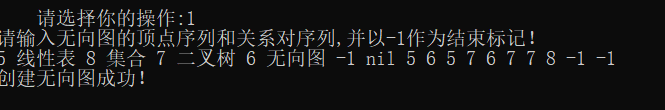
\includegraphics[width=\linewidth]{images/2.4.1.png}} \end{minipage}              &创建无向图成功    \\ \hline
			定位顶点      & 8                                                          & \begin{minipage}[b]{0.3\columnwidth} \centering \raisebox{-.5\height}{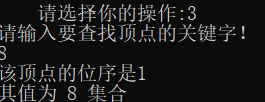
\includegraphics[width=\linewidth]{images/2.4.2.png}} \end{minipage}              &返回关键字为8的顶点的位序1    \\ \hline
			修改顶点      & 6 9 有向图                                                         & \begin{minipage}[b]{0.3\columnwidth} \centering \raisebox{-.5\height}{
\includegraphics[width=\linewidth]{images/2.4.4.png}} \end{minipage}              &修改成功    \\ \hline
			查找第一邻接点     & 7                                                          & \begin{minipage}[b]{0.3\columnwidth} \centering \raisebox{-.5\height}{
\includegraphics[width=\linewidth]{images/2.4.6.png}} \end{minipage}              &该顶点的第一邻接顶点的位序为1  其值为8 集合   \\ \hline
			查找下一邻接点     & 7 8                                                          & \begin{minipage}[b]{0.3\columnwidth} \centering \raisebox{-.5\height}{
\includegraphics[width=\linewidth]{images/2.4.9.png}} \end{minipage}              &顶点7的邻接顶点相对于8的下一邻接顶点的位序是3
			其值为 6 无向图    \\ \hline
			深度优先遍历     & 11                                                        & \begin{minipage}[b]{0.3\columnwidth} \centering \raisebox{-.5\height}{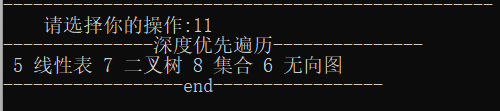
\includegraphics[width=\linewidth]{images/2.4.10.png}} \end{minipage}              & 5 线性表 7 二叉树 8 集合 6 无向图   \\ \hline
			广度优先遍历      & 12                                                          & \begin{minipage}[b]{0.3\columnwidth} \centering \raisebox{-.5\height}{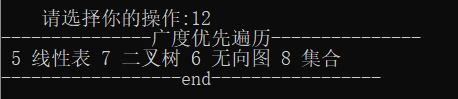
\includegraphics[width=\linewidth]{images/2.4.11.png}} \end{minipage}              & 5 线性表 7 二叉树 6 无向图 8 集合   \\ \hline
			销毁图      & 2                                                          & \begin{minipage}[b]{0.3\columnwidth} \centering \raisebox{-.5\height}{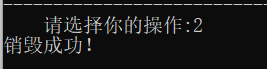
\includegraphics[width=\linewidth]{images/2.4.12.png}} \end{minipage}              &销毁成功    \\ \hline
		\end{tabular}
	}
\end{table}
\clearpage

表\ref{table3.4}为异常样例的输入,实际输出和对输出结果的分析\par

\begin{table}[htbp]
	\centering
	\caption{异常样例测试}
	\label{table3.4}
	\scalebox{0.7}{
		\begin{tabular}{|l|l|l|l|}
			\hline
			异常样例    & 输入            & 实际输出                                                                 & 结果分析       \\ \hline
			创建图      & 5 (略) 5 6 5 7 6 7 7 8 -1 -1                                                         & \begin{minipage}[b]{0.3\columnwidth} \centering \raisebox{-.5\height}{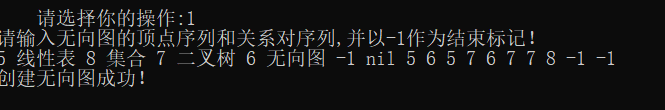
\includegraphics[width=\linewidth]{images/2.4.1.png}} \end{minipage}              &创建无向图成功    \\ \hline
			定位顶点      & 10                                                          & \begin{minipage}[b]{0.3\columnwidth} \centering \raisebox{-.5\height}{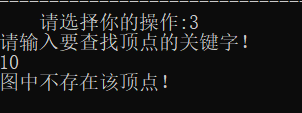
\includegraphics[width=\linewidth]{images/2.4.3.png}} \end{minipage}              &找不到关键字为10的顶点    \\ \hline
			修改顶点      & 6 5 有向图                                                        & \begin{minipage}[b]{0.3\columnwidth} \centering \raisebox{-.5\height}{
\includegraphics[width=\linewidth]{images/2.4.5.png}} \end{minipage}              &关键字为5的结点已存在   \\ \hline
			查找第一邻接点 & 10                                                           & \begin{minipage}[b]{0.3\columnwidth} \centering \raisebox{-.5\height}{
\includegraphics[width=\linewidth]{images/2.4.8.png}} \end{minipage}                     &找不到关键字为10的顶点  \\ \hline  
			销毁图 & 2                                                           & \begin{minipage}[b]{0.3\columnwidth} \centering \raisebox{-.5\height}{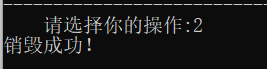
\includegraphics[width=\linewidth]{images/2.4.12.png}} \end{minipage}                     &销毁成功  \\ \hline    
			销毁图 & 2                                                           & \begin{minipage}[b]{0.3\columnwidth} \centering \raisebox{-.5\height}{
\includegraphics[width=\linewidth]{images/2.4.13.png}} \end{minipage}                     &图还未创建,无法销毁  \\ \hline         
		\end{tabular}
	}
\end{table}

通过异常用例可以看出,演示系统对要求插入与已有顶点关键字相同的顶点,和定位不包含在图中的顶点以及销毁还未创建的图等操作的判定能力,可见演示系统能够识别异常样例。
\clearpage
\subsection{实验小结}
本次实验让我对基于邻接表的图实现的了解更进了一步。\\
演示系统的搭建,让我体会到了主函数和子函数的关系,以及如何搭建一个可以调用不同模块的系统。\par
在编写插入和删除弧的函数时,如何有效地根据关键字找到相应结点是使程序变得简介的一大关键,在编写插入与删除弧的函数时,如果能够在之前定义定位顶点的函数,并调用,将极大地省去冗杂的代码,这次实验让我对函数的工具性,模块性有了直观的感受。\par
总的来说,本次数据结构实验提高了我的编程能力,让我对系统整体设计有了更深的认识。\par
相比之前几次的实验,图的系统实现更为复杂,进阶操作的实现需要了解一些经典的算法,本次实验让我有了较大的进步。
\clearpage
\section{课程的收获和建议}
\subsection{基于链式存储结构的线性表实现}
通过对基于链式存储结构的线性表实现的演示系统练习,我基本掌握了线性表的基本操作,能够根据需要调用不同的模块来灵活地使用线性表这一数据结构。\par
同时在实验过程中,尤其是在debug的过程中,我明白了看书看懂了并不代表自己就掌握了一种数据结构,实际上还差的很远,唯有动手实践,多用样例测试,才能了解与熟练运用它。\par
许许多多的细节问题不通过实践,是无法学到的。
\subsection{基于邻接表的图实现}
数据结构这门课里最复杂的数据结构就是图,通过对基于邻接表的图实现的实验学习,我对数据结构的认识更进了一步。\par
这门课程可以说是计算机专业的基础课程,也是核心课程。\par
经过一学期的学习,我希望未来数据结构课能够越来越好。\par
\nocite{*} %% 作用是不对文献进行引用,但可以生成文献列表

\bibliographystyle{Experimental Report}
\bibliography{Experimental Report}
\setcounter{secnumdepth}{0}
\appendix
		\section{附录A 基于链式存储结构线性表实现的源程序}
		\begin{lstlisting}[language=C] 
			#include<stdio.h>
#include<malloc.h>
#include<stdlib.h>
#include<string.h>

#define TRUE 1
#define FALSE 0
#define OK 1
#define ERROR 0
#define INFEASIBLE -1
#define OVERFLOW -2

typedef int status;
typedef int ElemType; 数据元素类型定义

#define LIST INIT SIZE 100
#define LISTINCREMENT  10

typedef int ElemType;
typedef struct LNode{单链表(链式结构)结点的定义
	ElemType data;
	struct LNode* next;
}LNode, *LinkList;

status InitList(LinkList& L);
status DestroyList(LinkList& L);
status ClearList(LinkList& L);
status ListEmpty(LinkList L);
status ListLength(LinkList L);
status GetElem(LinkList L, int i, ElemType& e);
status LocateElem(LinkList L, ElemType e);
status PriorElem(LinkList L, ElemType e, ElemType& pre);
status NextElem(LinkList L, ElemType e, ElemType& next);
status ListInsert(LinkList& L, int i, ElemType e);
status ListDelete(LinkList& L, int i, ElemType& e);
status ListTraverse(LinkList L);

status SaveList(LinkList L, char FileName[]);
status LoadList(LinkList& L, char FileName[]);
status AddList(LISTS& lists);
status RemoveList(LISTS& Lists, char name[]);
status LocateList(LISTS Lists, char name[]);
status ReverseList(LinkList &L);
status RemoveNthFromEnd(LinkList L, int n, ElemType& e);
status SortList(LinkList L);

int main()
{
	int op = 1, flag ,length, next, pre, i, e, n;
	LISTS Lists;
	LIST* temp;
	if(!(Lists.head = (LIST *)malloc(sizeof(LIST))))
	exit(OVERFLOW);
	if (!(Lists.head -> head = (LinkList)malloc(sizeof(LNode))))
	exit(OVERFLOW);
	Lists.head -> head -> data = 0;
	Lists.head -> next = NULL;
	char name[25];
	LinkList L = NULL;
	while(op){
		system("cls");	清屏
printf("\n");	打印指令集
printf("      Menu for Linear Table On Sequence Structure \n");
printf("-------------------------------------------------\n");
printf("	  1. InitList             2. DestroyList\n");
printf("	  3. ClearList            4. ListEmpty\n");
printf("	  5. ListLength           6. GetElem\n");
printf("	  7. LocateElem           8. PriorElem\n");
printf("	  9. NextElem             10. ListInsert\n");
printf("	  11. ListDelete          12. ListTrabverse\n");
printf("\n"); 
printf("	  13.SaveList             14. LoadList\n");
printf("	  15.SortList            16.ReverseList\n");
printf("	  17.RemoveNthFromEnd\n");
printf("          0. exit\n");
printf("-------------------------------------------------\n");
printf("    请选择你的操作[0~17]:\n");
		scanf("%d", &op);
					switch(op){
	case 1:	创建线性表
	if(InitList(L) == OK)
	printf("线性表创建成功\n");
	else
	printf("线性表创建失败\n");
	getchar(); getchar();
	break;
	case 2:	销毁线性表
	if(DestroyList(L) == OK)
	printf("线性表销毁成功\n");
	else
	printf("线性表不存在\n");
	getchar(); getchar();
	break;
	case 3:	删除线性表
	if(ClearList(L) == OK)
	printf("线性表清空成功\n");
	else
	printf("线性表不存在\n");
	getchar(); getchar();
	break;
	case 4:	判空
	flag = ListEmpty(L);
	if(flag == TRUE)
	printf("线性表为空\n");
	else if(flag == FALSE)
	printf("线性表不为空\n");
	else
	printf("线性表不存在!\n");
	getchar(); getchar();
	break;
	case 5:	求表长
	length = ListLength(L);
	if(length != INFEASIBLE)
	printf("线性表长度为%d\n", length);
	else
	printf("线性表不存在\n");
	getchar(); getchar();
	break;
	case 6:	获取元素
	if(!L)
	printf("线性表不存在\n");
	else{
		printf("想要获取第几个元素:");
		scanf("%d", &i);
		flag = GetElem(L, i, e);
		if(flag == OK)
		printf("获取元素为%d\n", e);
		else if(flag == ERROR)
		printf("位置不合法\n");
		else
		printf("线性表不存在\n");
	}
	getchar(); getchar();
	break;
	case 7:	定位元素
	if(!L)
	printf("线性表不存在\n");
	else{
		printf("请输入元素:");
		scanf("%d", &e);
		if((i = LocateElem(L, e)) != 0)
		printf("元素位置为%d\n", i);
		else if (i == ERROR)
		printf("查找元素位置失败\n");
		else
		printf("线性表不存在\n");
	}
	getchar(); getchar();
	break;
	case 8:	查找前驱
	if(!L)
	printf("线性表不存在\n");
	else{
		printf("请输入元素:");
		scanf("%d", &e);
		flag = PriorElem(L, e, pre);
		if(flag == OK)
		printf("元素的前驱为%d\n", pre);
		else if(flag == ERROR)
		printf("查找前驱失败\n");
		else printf("线性表为空\n");
	}
	getchar(); getchar();
	break;
	case 9:	查找后继
	if(!L)
	printf("线性表不存在\n");
	else {
		printf("请输入元素:");
		scanf("%d", &e);
		flag = NextElem(L, e, next);
		if(flag == OK)
		printf("元素的后继为%d\n", next);
		else if(flag == ERROR)
		printf("查找后继元素失败\n");
		else
		printf("线性表为空\n");
	}
	getchar(); getchar();
	break;
	case 10:	插入元素
	if(!L)
	printf("线性表不存在\n");
	else{
		scanf("%d",&i);
		scanf("%d",&e);
		flag = ListInsert(L, i, e);
		if(flag == OK)
		printf("插入成功\n");
		else if(flag == ERROR)
		printf("插入位置不合法\n");
	}
	getchar(); getchar();
	break;
	case 11:	删除元素
	if(!L)
	printf("线性表不存在\n");
	else{
		printf("想要删除第几个元素:");
		scanf("%d", &i);
		flag = ListDelete(L, i, e);
		if(flag == OK)
		printf("删除成功,被删除的元素为:%d\n", e);
		else if(flag == ERROR)
		printf("删除位置不合法\n");
		else
		printf("线性表为空\n");
	}
	getchar(); getchar();
	break;
	case 12:    遍历
	if(!L)
	printf("线性表不存在\n");
	else{
		ListTraverse(L);
		printf("遍历完成\n");
	}
	getchar(); getchar();
	break;
	case 13:	写入文件
	if(!L)
	printf("线性表不存在\n");
	else{
		printf("请输入文件名:\n");
		scanf("%s", name);
		flag = SaveList(L, name);
		if(flag == OK)
		printf("保存文件成功\n");
		else
		printf("保存文件失败\n");
	}
	getchar(); getchar();
	break;
	case 14:	读入文件
	if(L)
	printf("该线性表已存在,不可读入");
	else{
		printf("请输入文件名:");
		scanf("%s", name);
		flag = LoadList(L, name);
		if (flag == OK)
		printf("读入文件成功\n");
		else
		printf("读入文件失败\n");
	}
	getchar(); getchar();
	break;
	case 15:
	flag = SortList(L);
	if(flag == INFEASIBLE) printf("线性表不存在\n");
	else if(flag == ERROR) printf("线性表为空\n");
	else{
		SortList(L);
		printf("排序成功\n");
	}
	getchar(); getchar();
	break;
	case 16:
	flag = ReverseList(L);
	if(flag == INFEASIBLE) printf("线性表不存在\n");
	else if(flag == ERROR) printf("线性表为空\n");
	else printf("翻转成功\n");
	getchar(); getchar();
	break;
	case 17:
	printf("请问你想删除倒数第几个元素:\n");
	scanf("%d", &n);
	flag = RemoveNthFromEnd(L, n, e);
	if(flag == INFEASIBLE) printf("线性表不存在\n");
	else if(flag == ERROR) printf("线性表为空\n");
	else
	{
		printf("删除成功\n");
	}
	getchar(); getchar();
	break;
	case 0:	结束程序
	break;
}end of switch
}end of while
printf("欢迎下次再使用本系统!\n");
return 0;
}end of main()


status InitList(LinkList &L)
线性表L不存在,构造一个空的线性表,返回OK,
否则返回INFEASIBLE。
{
请在这里补充代码,完成本关任务
Begin  
if(L) return INFEASIBLE;
L=(LNode*)malloc(sizeof(LNode));
L->next=NULL;
if(L) return OK;
End  
}

status DestroyList(LinkList &L)
如果线性表L存在,销毁线性表L,释放数据元素的空间,返回OK,
否则返回INFEASIBLE。
{
请在这里补充代码,完成本关任务
Begin  
if(!L) return INFEASIBLE;
LinkList p;
while(L)
{
p=L;
L=L->next;
free(p);
}
return OK;
End  
}

status ClearList(LinkList &L)
{
请在这里补充代码,完成本关任务
Begin  
if(!L) return INFEASIBLE;
LinkList p;
while(L->next)
{
p=L->next;
L->next=p->next;
free(p);
}
return OK;
End  
}

status ListEmpty(LinkList L)
如果线性表L存在,判断线性表L是否为空,空就返回TRUE,否则返回FALSE;
如果线性表L不存在,返回INFEASIBLE。
{
请在这里补充代码,完成本关任务
Begin  
if(!L) return INFEASIBLE;
if(!L->next) return TRUE;
else return FALSE;

End  
}


int ListLength(LinkList L)
如果线性表L存在,返回线性表L的长度,否则返回INFEASIBLE。
{
请在这里补充代码,完成本关任务
Begin  
if(!L) return INFEASIBLE;
int ans=0;
LinkList p=L;
while(p->next)
{
ans++;
p=p->next;
}
return ans;
End  
}
			
			
status GetElem(LinkList L,int i,ElemType &e)
{
	请在这里补充代码,完成本关任务
	Begin  
	if(!L) return INFEASIBLE;
	if(i<=0) return ERROR;
	LinkList p=L;
	for(int j=0;j<i;j++)
	{
		p=p->next;
		if(!p) return ERROR;
	}
	e=(*p).data;
	return OK;
	End  
}

status LocateElem(LinkList L,ElemType e)
{
	请在这里补充代码,完成本关任务
	Begin  
	if(!L) return INFEASIBLE;
	LinkList p=L->next;
	int ans=1;
	while(p)
	{  
		if((*p).data==e) return ans;
		ans++;
		p=p->next;
	}
	return ERROR;
	End  
}

status PriorElem(LinkList L,ElemType e,ElemType &pre)
如果线性表L存在,获取线性表L中元素e的前驱,保存在pre中,返回OK;
如果没有前驱,返回ERROR;如果线性表L不存在,返回INFEASIBLE。
{
	请在这里补充代码,完成本关任务
	Begin  
	if(!L) return INFEASIBLE;
	LinkList p=L->next;
	LinkList q=L;
	int ans=0;
	while(p)
	{  
		if((*p).data==e) 
		{
			if(!ans) return ERROR;
			pre=(*q).data;
			return OK;
		}
		ans++;
		p=p->next;
		q=q->next;
	}
	return ERROR;
	End  
}


status NextElem(LinkList L,ElemType e,ElemType &next)
如果线性表L存在,获取线性表L元素e的后继,保存在next中,返回OK;
如果没有后继,返回ERROR;如果线性表L不存在,返回INFEASIBLE。
{
	请在这里补充代码,完成本关任务
	Begin  
	if(!L) return INFEASIBLE;
	LinkList p=L->next;
	if(!p) return ERROR;
	LinkList q=p->next;
	while(q)
	{  
		if((*p).data==e) 
		{
			next=(*q).data;
			return OK;
		}
		p=p->next;
		q=q->next;
	}
	return ERROR;
	End  
}

status ListInsert(LinkList &L,int i,ElemType e)
如果线性表L存在,将元素e插入到线性表L的第i个元素之前,返回OK;
当插入位置不正确时,返回ERROR;如果线性表L不存在,返回INFEASIBLE。
{
	请在这里补充代码,完成本关任务
	Begin  
	if(!L) return INFEASIBLE;
	LinkList p=L,q;
	if(!L->next)
	{
		if(i!=1) return ERROR;
		p->next=(LNode*)malloc(sizeof(LNode));
		p=p->next;
		(*p).data=e;
		p->next=NULL;
		return OK;
	} 
	q=L->next;
	if(i<=0) return ERROR;
	for(int ans=1;ans<i;ans++)
	{  
		p=p->next;
		if(q) q=q->next;
		else return ERROR;
	}
	p->next=(LNode*)malloc(sizeof(LNode));
	p=p->next;
	(*p).data=e;
	p->next=q;
	return OK;
	End  
}

status ListDelete(LinkList &L,int i,ElemType &e)
如果线性表L存在,删除线性表L的第i个元素,并保存在e中,返回OK;
当删除位置不正确时,返回ERROR;如果线性表L不存在,返回INFEASIBLE。
{
	请在这里补充代码,完成本关任务
	Begin  
	if(!L) return INFEASIBLE;
	LinkList p=L,q;
	int ans=1;
	if(L->next) q=L->next;
	if(i<=0) return ERROR;
	for(ans;ans<i;ans++)
	{  
		p=p->next;
		if(q->next) q=q->next;
		else return ERROR;
	}
	p->next=q->next;
	e=(*q).data;
	free(q);
	return OK;
	End  
}

status ListTraverse(LinkList L)
如果线性表L存在,依次显示线性表中的元素,每个元素间空一格,返回OK;
如果线性表L不存在,返回INFEASIBLE。
{
	请在这里补充代码,完成本关任务
	Begin  
	if(!L) return INFEASIBLE;
	LinkList p=L;
	while(p->next)
	{
		p=p->next;
		printf("%d ",(*p).data);
	}
	return OK;
	End  
}

status SaveList(LinkList L,char FileName[])
如果线性表L存在,将线性表L的的元素写到FileName文件中,返回OK,
否则返回INFEASIBLE。
{
	请在这里补充代码,完成本关任务
	Begin 1  
	if(!L)
	{
		return INFEASIBLE;
	}
	else
	{
		LinkList p=L;
		FILE *fp=fopen(FileName,"w+");
		if(!fp) return ERROR;
		while(p->next)
		{
			p=p->next;
			fprintf(fp,"%d ",(*p).data);
		}
		fclose(fp);
		return OK;
	}
	End 1  
}

status LoadList(LinkList &L,char FileName[]) 
如果线性表L不存在,将FileName文件中的数据读入到线性表L中,返回OK,
否则返回INFEASIBLE。
{
	请在这里补充代码,完成本关任务
	Begin 2  
	if(L) return INFEASIBLE;
	L=(LNode*)malloc(sizeof(LNode));
	FILE *fp=fopen(FileName,"r");
	if(!fp) return ERROR;
	ElemType e;
	LinkList p=L;
	while((fscanf(fp,"%d",&e))==1)
	{
		p->next=(LNode*)malloc(sizeof(LNode));
		p=p->next;
		(*p).data=e;
	}
	p->next=NULL;
	fclose(fp);
	return OK;
	End 2  
}

status ReverseList(LinkList &L)
如果线性表L存在,翻转线性表,返回OK;如果不存在,返回INFEASIBLE。
{
	if(L)
	{
		LinkList p,q;
		if(L -> next == NULL)  return ERROR;
		p = L -> next;
		q = L -> next -> next;
		while(q != NULL)
		{
			p -> next = q -> next;
			q -> next = L -> next;
			L -> next = q;
			q = p -> next;
		}
		return OK;
	}
	else  return INFEASIBLE;
}

status RemoveNthFromEnd(LinkList L, int n, ElemType& e)
{
	if(!L) return INFEASIBLE;
	else
	{
		int k,j; 
		if(L->next==NULL) return ERROR;
		k = ListLength(L);
		j = k - n + 1;
		ListDelete(L, j, e);
		return OK;
	}
}

status SortList(LinkList L)
{
	LinkList p, q;
	if(!L) return INFEASIBLE;
	else{
		if(L->next==NULL) return ERROR;
		int n = ListLength(L);
		int i, j, temp;
		for(i = 0,p = L -> next; i < n-1; i++,p = p -> next)
		{
			for(j = i + 1,q = p -> next; j < n; j++,q = q -> next)
			{
				if(p -> data > q -> data)
				{
					temp = p -> data;
					p -> data = q -> data;
					q -> data = temp;
				}
			}
		}
		return OK;
	}
}
\end{lstlisting}
\newpage
\section{附录B 基于邻接表图实现的源程序}
		\begin{lstlisting}[language=C] 
#include "stdio.h"
#include "stdlib.h"
#include<string.h>
#define TRUE 1
#define FALSE 0
#define OK 1
#define ERROR 0
#define INFEASIBLE -1
#define OVERFLOW -2
#define MAX_VERTEX_NUM 20
typedef int status;
typedef int KeyType; 
typedef enum {DG,DN,UDG,UDN} GraphKind;
typedef struct {
	KeyType  key;
	char others[20];
} VertexType; 顶点类型定义
typedef struct ArcNode {      
	int adjvex;            
	struct ArcNode  *nextarc;	   
} ArcNode;
typedef struct VNode{		
	VertexType data;       
	ArcNode *firstarc;      	 
} VNode,AdjList[MAX_VERTEX_NUM];
typedef  struct {  邻接表的类型定义
	AdjList vertices;     	
	int vexnum,arcnum;   	  
	GraphKind  kind;       
} ALGraph;
struct ptr{
	void *pused[100],*pfree[100];
	int len_used,len_free;
} pm;
typedef struct QNode{
	VertexType data;
	struct QNode *next;
}QNode,*Queue;
typedef struct{
	Queue front;
	Queue rear;
}Linkqueue;
void free0(void *p)
{
	pm.pfree[pm.len_free++]=p;
	memset(p,0,sizeof(ArcNode));
	free(p);
}
bool visited[MAX_VERTEX_NUM];
int pd;
void visit(VertexType v)
{
	printf(" %d %s",v.key,v.others);
}
status issame(VertexType V[])判断顶点重复 
{
	int i=0;
	int mark[100000]={0};
	while(V[i].key!=-1)
	{
		if(mark[V[i].key]>0){return 1;}
		mark[V[i].key]++;
		i++;
	}
	return 0;
}
int Locate (ALGraph G,KeyType VR)
{
	int i=0;
	for(i;i<G.vexnum;i++)
	{
		if(G.vertices[i].data.key==VR) return i;
	}
	return -1;
}
status CreateCraph(ALGraph &G,VertexType V[],KeyType VR[][2])
{
	int i=0,j=0;
	while(V[i].key!=-1)
	{
		for(int k=0;k<i;k++)
		{
			if(V[i].key==V[k].key) return ERROR;
		}
		if(i>=MAX_VERTEX_NUM) return ERROR;
		G.vertices[i].data=V[i];
		G.vertices[i].firstarc=NULL;
		i++;
	}
	if(i==0) return ERROR;
	G.vexnum=i;
	while(VR[j][0]!=-1)
	{
	int a=Locate(G,VR[j][0]),b=Locate(G,VR[j][1]);
if(!(a>=0&&b>=0)) return ERROR;
ArcNode *q=(ArcNode*)malloc(sizeof(ArcNode)) ;
q->adjvex=b;
q->nextarc=G.vertices[a].firstarc;
G.vertices[a].firstarc=q;
q=(ArcNode*)malloc(sizeof(ArcNode)) ;
q->adjvex=a;
q->nextarc=G.vertices[b].firstarc;
G.vertices[b].firstarc=q;
j++;
	}
	G.arcnum=j;
}

status DestroyGraph(ALGraph &G)
{

ArcNode *p=NULL,*q=NULL;
for(int k=0;k<G.vexnum;k++)
{
	if(G.vertices[k].firstarc!=NULL)
	{
		p=G.vertices[k].firstarc;
		while(p!=NULL)
		{
			q=p->nextarc;
			free(p);
			p=q;
		}
		G.vertices[k].firstarc=NULL;
	}
}
	G.arcnum=0;
	G.vexnum=0;
	return OK;
}

int LocateVex(ALGraph G,KeyType u)
{
	int i=0;
	for(i;i<G.vexnum;i++)
	{
		if(G.vertices[i].data.key==u) return i;
	}
	return -1;
	

}
status PutVex(ALGraph &G,KeyType u,VertexType value)

{
	int i=0;
	for(i;i<G.vexnum;i++)
	{
		if(G.vertices[i].data.key==u) 
		{
	for(int k=0;k<G.vexnum;k++)
{
	if(G.vertices[k].data.key==value.key) return ERROR;
}
G.vertices[i].data=value;  return OK;
		}
	}
	return ERROR;  
	
}

int FirstAdjVex(ALGraph G,KeyType u)
{
	int i=0;
	for(i;i<G.vexnum;i++)
	{
	if(G.vertices[i].data.key==u) 
{
	return G.vertices[i].firstarc->adjvex;
}
	}
	return -1;
	
}

int NextAdjVex(ALGraph G,KeyType v,KeyType w)
{
	int i=LocateVex(G,v),j=LocateVex(G,w);
	while(i!=-1&&j!=-1)
	{
		ArcNode *p=G.vertices[i].firstarc;
		while(p->adjvex!=j&&p)
		{
			p=p->nextarc;
		}
		if(p->nextarc)
		{
			return p->nextarc->adjvex;
		}
		else return -1;
	}
	return -1;
	
}
status InsertVex(ALGraph &G,VertexType v)
{
	if(LocateVex(G,v.key)>=0) return ERROR;
	if(G.vexnum==MAX_VERTEX_NUM) return ERROR;
	G.vertices[G.vexnum].data=v;
	G.vertices[G.vexnum].firstarc=NULL;
	G.vexnum++;
	return OK;
}


status DeleteVex(ALGraph &G,KeyType v)
{
	int i=LocateVex(G,v),j=-1;
	if(i==-1) return ERROR;
	if(G.vexnum==1 || G.vexnum==0)return ERROR;
	ArcNode *p=G.vertices[i].firstarc;
	ArcNode *q=NULL;
	ArcNode *temp=NULL;
	while(p)
	{  
		j=p->adjvex;
		q=G.vertices[j].firstarc;
		if(q->adjvex==i)
		{
			temp=q;
			G.vertices[j].firstarc=q->nextarc;
			free(temp); 
		}
		else
		{
			while(q->nextarc->adjvex!=i)
			{
				q=q->nextarc;
			}
			temp=q->nextarc;
			q->nextarc=temp->nextarc;
			free(temp);
		}
		temp=p->nextarc;
		free(p);
		p=temp;
		G.arcnum--;
	}
	for(int k=i;k<G.vexnum;k++)
	{
		G.vertices[k]=G.vertices[k+1];
	}
	G.vexnum--;
	for(int k=0;k<G.vexnum;k++)
	{
		p=G.vertices[k].firstarc;
		while(p!=NULL)
		{
			if(p->adjvex>i)
			p->adjvex--;
			p=p->nextarc;
		}
	}
	return OK;
}
status Locatearc(ALGraph G,KeyType v,KeyType w)
{
	ArcNode *p=G.vertices[v].firstarc;
	while(p!=NULL)
	{
		if(p->adjvex==w)
		return OK;
		p=p->nextarc;
	}
	return ERROR;
}
int LocateArc(ALGraph G,KeyType v,KeyType w)
{
	int i=LocateVex(G,v);
	int j=LocateVex(G,w);
	if(i==-1||j==-1) return ERROR;
	ArcNode *p=G.vertices[i].firstarc;
	while(p!=NULL)
	{
		if(p->adjvex==j)
		return OK;
		p=p->nextarc;
	}
	return ERROR;
}
status InsertArc(ALGraph &G,KeyType v,KeyType w)
{

	int i=LocateVex(G,v);
	int j=LocateVex(G,w);
	if(i==-1||j==-1) return ERROR;
	if(LocateArc(G,v,w)!=ERROR) return ERROR;
	ArcNode *p=(ArcNode*)malloc(sizeof(ArcNode));
	p->adjvex=j;
	p->nextarc=G.vertices[i].firstarc;
	G.vertices[i].firstarc=p;
	p=(ArcNode*)malloc(sizeof(ArcNode));
	p->adjvex=i;
	p->nextarc=G.vertices[j].firstarc;
	G.vertices[j].firstarc=p;
	G.arcnum++;
	return OK;
}
status DeleteArc(ALGraph &G,KeyType v,KeyType w)
{
	if(LocateArc(G,v,w)==ERROR) return ERROR;
	int i=LocateVex(G,v);
	int j=LocateVex(G,w);
	ArcNode *p=G.vertices[i].firstarc;
	ArcNode *temp=NULL;
	if(p->adjvex==j)
	{
		temp=p;
		G.vertices[i].firstarc=p->nextarc;
		free(temp);
	}
	else 
	{
		while(p->nextarc->adjvex!=j)
		{
			p=p->nextarc;
		}
		temp=p->nextarc;
		p->nextarc=p->nextarc->nextarc;
		free(temp);
	}
	p=G.vertices[j].firstarc;
	temp=NULL;
	if(p->adjvex==i)
	{
		temp=p;
		G.vertices[j].firstarc=p->nextarc;
		free(temp);
	}
	else 
	{
		while(p->nextarc->adjvex!=i)
		{
			p=p->nextarc;
		}
		temp=p->nextarc;
		p->nextarc=p->nextarc->nextarc;
		free(temp);
	}
	G.arcnum--;
	return OK;
}
void dfs(ALGraph &G,KeyType v,void(*visit)(VertexType))
{
	visited[v]=TRUE;
	int x=LocateVex(G,v);
	visit(G.vertices[x].data);
for(int w=FirstAdjVex(G,v);w>=0;
w=NextAdjVex(G,v,G.vertices[w].data.key)) 
{
	if(!visited[G.vertices[w].data.key])
	dfs(G,G.vertices[w].data.key,
	visit);
}
}
status DFSTraverse(ALGraph &G,void(*visit)(VertexType))
{
	int i;
	for(i=0;i<G.vexnum;i++)
	visited[G.vertices[i].data.key]=FALSE;标记数组记录关键字 
	for(i=0;i<G.vexnum;i++)
	{
		if(!visited[G.vertices[i].data.key])
		{
			dfs(G,G.vertices[i].data.key,visit);
			
		}
	}
	return OK;
} 
			status InitQueue(Linkqueue &Q)
{
Q.front=Q.rear=(QNode *)malloc(sizeof(QNode));
	if(!Q.front)return ERROR;
	Q.front->next=NULL;
	return OK;
} 
status QueueEmpty(Linkqueue Q)
{
	if(Q.front==Q.rear)return TRUE;
	else return FALSE;
}
status enQueue(Linkqueue &Q,VertexType value)
{
	Queue p=(Queue)malloc(sizeof(QNode));
	if(!p)return ERROR;
	p->data=value;
	p->next=NULL;
	Q.rear->next=p;
	Q.rear=p;
	return OK;
}
status deQueue(Linkqueue &Q,VertexType &value)
{
	if(Q.front==Q.rear)return ERROR;
	Queue p=Q.front->next;
	value=p->data;
	Q.front->next=p->next;
	if(Q.rear==p)
	Q.rear=Q.front;
	free(p);
	return OK;
}
status BFSTraverse(ALGraph &G,void (*visit)(VertexType))
对图G进行广度优先搜索遍历,依次对图中的每一个顶点使用函数visit访问一次,且仅访问一次
{
	int i=0,j;
	VertexType value;
	Linkqueue Q;
	InitQueue(Q);
	for(i=0;i<G.vexnum;i++)
	{
		visited[G.vertices[i].data.key]=FALSE;
	}
	for(i=0;i<G.vexnum;i++)
	{
		if(!visited[G.vertices[i].data.key])
		{
	visited[G.vertices[i].data.key]=TRUE;
visit(G.vertices[i].data);
enQueue(Q,G.vertices[i].data);
while(!QueueEmpty(Q))
{
deQueue(Q,value);
for(int w=FirstAdjVex(G,value.key);w>=0;
w=NextAdjVex(G,value.key,G.vertices[w].data.key))
{
	if(!visited[G.vertices[w].data.key])
	{
		visited[G.vertices[w].data.key]=TRUE;
		visit(G.vertices[w].data);
		enQueue(Q,G.vertices[w].data);
	}
} 
}
		}
	}
	return OK;
}
status SaveGraph(ALGraph G, char FileName[])
将图的数据写入到文件FileName中
{
	FILE *fp=fopen(FileName,"w");
	fprintf(fp,"%d %d ",G.vexnum,G.arcnum);
	int i=0;
	for(i=0;i<G.vexnum;i++)
	{
		fprintf(fp,"%d,%s ",G.vertices[i].data.key,
		G.vertices[i].data.others);
		ArcNode *p=G.vertices[i].firstarc;
		while(p!=NULL)
		{
			fprintf(fp,"%d ",p->adjvex);
			p=p->nextarc;
		}
		fprintf(fp,"%d ",-1);
	}
	fclose(fp);
	return OK;
}
#include<string.h>
status LoadGraph(ALGraph &G, char FileName[])
读入文件FileName的图数据,创建图的邻接表
{
	FILE *fp=fopen(FileName,"r");
	char c,d;
	char other[20];
	int i,j,k;
	fscanf(fp,"%d%d",&G.vexnum,&G.arcnum);
	for(i=0;i<G.vexnum;i++)
	{
		fscanf(fp,"%d%c%s",&k,&c,other);
		G.vertices[i].data.key=k;
		strcpy(G.vertices[i].data.others,other);
		j=0;
		ArcNode *rear=G.vertices[i].firstarc=NULL;
		while(j!=-1)
		{
			fscanf(fp,"%d",&j);
			if(j!=-1){
	ArcNode *p=(ArcNode *)malloc(sizeof(ArcNode));
		p->adjvex=j;
		p->nextarc=NULL;
		if(G.vertices[i].firstarc==NULL)
		{
			G.vertices[i].firstarc=p;
			rear=G.vertices[i].firstarc;
		}
		else{
			rear->nextarc=p;
			rear=p;
				}
			}
		}
		rear=NULL;
	}
	fclose(fp);
	return OK;
}
			int distance[21];
status ShortestPathLength(ALGraph G,KeyType v,KeyType w)返回顶点v与顶点w的最短路径长度 
{
	int i,j,n;
	VertexType top;
	top.key=v;
	Linkqueue Q;
	InitQueue(Q);
	for(i=0;i<G.vexnum;i++)
	distance[G.vertices[i].data.key]=20;
	distance[v]=0;
	int k=LocateVex(G,v);
	enQueue(Q,G.vertices[k].data);
	while(!QueueEmpty(Q))
	{
deQueue(Q,top);
if(top.key==w)break;
for(j=FirstAdjVex(G,top.key);
j>=0;j=NextAdjVex(G,top.key,G.vertices[j].data.key))
{
	if(distance[G.vertices[j].data.key]==20)
{
	distance[G.vertices[j].data.key]=distance[top.key]+1;
	enQueue(Q,G.vertices[j].data);
}
}
	}
	n=distance[w];
	return n;
}
void VerticesSetLessThank(ALGraph G,KeyType v,KeyType k)
{
	int i,j;
for(i=0;i<G.vexnum;i++)
{
	j=ShortestPathLength(G,v,G.vertices[i].data.key);
	if(j<k&&G.vertices[i].data.key!=v)
	visit(G.vertices[i].data);
}
}
bool mark[20];
void dfs(ALGraph &G,KeyType v)
{
	mark[v]=TRUE;
for(int w=FirstAdjVex(G,v);
w>=0;w=NextAdjVex(G,v,G.vertices[w].data.key)) 
{
	if(!mark[G.vertices[w].data.key])
	dfs(G,G.vertices[w].data.key);
}
}
status ConnectedComponentsNums(ALGraph G)
{
	int count=0,i;
	for(i=0;i<G.vexnum;i++)
	mark[G.vertices[i].data.key]=FALSE; 
	for(i=0;i<G.vexnum;i++)
	{
		if(!mark[G.vertices[i].data.key])
		{
			dfs(G,G.vertices[i].data.key);
			count++;
		}
	}
	return count;
} 
int main(){
	int op=1,flag,x;
	ALGraph G;
	G.arcnum=0,G.vexnum=0;
	VertexType V[30];
	VertexType value;
	KeyType VR[100][2];
	int i=0,j,e,v,w,k;
	char filename[20];
	char name[20];
	while(op){
	system("cls");	printf("\n\n");
printf("      Menu for Linear Table On Sequence Structure \n");
printf("-------------------------------------------------\n");
printf("    	  1. CreateGraph                 2. DestroyGraph\n");
printf("    	  3. LocateVex                   4. PutVex\n");
printf("    	  5. FirstAdjVex                 6. NextAdjVex \n");
printf("    	  7. InsertVex                   8. DeleteVex\n");
printf("    	  9. InsertArc                   10. DeleteArc\n");
printf("    	  11. DFSTraverse                12. BFSTraverse\n");
printf("          13.VerticesSetLessThank        14.ShortestPathLength\n");
printf("          15.ConnectedComponentsNums     16.SaveGraph\n");
printf("          17.LoadGraph                   18.ArcTraverse\n");
printf("    	  19.AssignVex\n");
printf("    	  0.Exit\n");
printf("-------------------------------------------------\n");
printf("    请选择你的操作:");
scanf("%d",&op);
		switch(op){
			case 1:
i=0;
if(pd)printf("图已存在请先销毁!\n");
else{
	printf("请输入无向图的顶点序列和关系对序列,");
	printf("并以-1作为结束标记!\n"); 
	do {
		scanf("%d%s",&V[i].key,V[i].others);
	} while(V[i++].key!=-1);
	i=0;
	do{
		scanf("%d%d",&VR[i][0],&VR[i][1]);
	} while(VR[i++][0]!=-1);
	if(CreateCraph(G,V,VR)==OK)printf("创建无向图成功!\n");
	else printf("创建无向图失败!\n");
}
getchar();getchar();
break;
case 2:  
if(G.vexnum==0)printf("销毁失败,请先创建图!\n");
else{
	if(DestroyGraph(G)==OK)printf("销毁成功!\n");
	else printf("销毁失败,请先创建图!\n"); 
}
getchar();getchar();
break;
case 3:
if(G.vexnum==0)printf("图不存在!\n");
else{
	printf("请输入要查找顶点的关键字!\n");
	scanf("%d",&e);
	if(LocateVex(G,e)==-1)printf("图中不存在该顶点!\n");
	else 
	{
		x=LocateVex(G,e);
		printf("该顶点的位序是%d\n",x);
		printf("其值为 %d %s\n",G.vertices[x].data.key,
		G.vertices[x].data.others);
	}
}
getchar();getchar();
break;
case 4:
if(G.vexnum==0)printf("图不存在!\n");
else{
printf("请输入要修改顶点的关键字和修改后的关键字和值!\n");
	scanf("%d",&j);
	scanf("%d%s",&value.key,value.others);
	if(LocateVex(G,j)==-1 || LocateVex(G,j)==-2)
	printf("该顶点不存在!\n"); 
	else if(PutVex(G,j,value)==OK)printf("修改成功!\n");
	else printf("修改失败!\n");
}
getchar();getchar();
break;
case 5:
if(G.vexnum==0)printf("图不存在!\n");
else{
	printf("请输入要查找第一邻接顶点的关键字!\n");
	scanf("%d",&e);
	if(FirstAdjVex(G,e)==-1)printf("查找失败!\n");
	else{
		x=FirstAdjVex(G,e);
		printf("该顶点的第一邻接顶点的位序为%d\n",x);
printf("其值为%d %s\n",G.vertices[x].data.key,
G.vertices[x].data.others);
	}
}
getchar();getchar();
break;
case 6:
if(G.vexnum==0)printf("图不存在!\n");
else{
	printf("请输入要查找顶点和相对顶点的关键字!\n");
	scanf("%d%d",&v,&w);  
	if(NextAdjVex(G,v,w)==-1)printf("查找失败!\n");
	else {
x=NextAdjVex(G,v,w);
printf("顶点%d的邻接顶点相对于%d的下一邻接顶点的位序是%d\n",v,w,x);
printf("其值为 %d %s\n",G.vertices[x].data.key,G.vertices[x].data.others); 
	}
}
getchar();getchar();
break;
case 7:
printf("请输入要插入结点的值!\n");
scanf("%d%s",&value.key,value.others);
if(InsertVex(G,value)==OK)printf("插入成功!\n");
else printf("插入失败!\n");
getchar();getchar();
break;
case 8:
if(G.vexnum==0)printf("图不存在!\n");
else{
	printf("请输入要删除顶点的关键字!\n");
	scanf("%d",&v);
	if(DeleteVex(G,v)==OK)printf("删除成功!\n");
	else printf("删除失败!\n");
}
getchar();getchar();
break;
case 9:
if(G.vexnum==0)printf("图不存在!\n");
else{
	printf("请输入要插入弧对应的两个顶点!\n");
scanf("%d%d",&v,&w);
if(InsertArc(G,v,w)==OK)printf("插入弧成功!\n");
else printf("插入弧失败!\n");
}
getchar();getchar();
break;
case 10:
if(G.vexnum==0)printf("图不存在!\n");
else{
printf("请输入要删除弧对应的两个顶点!\n");
scanf("%d%d",&v,&w);
if(DeleteArc(G,v,w)==OK)printf("删除弧成功!\n");
else printf("删除弧失败!\n"); 
}
getchar();getchar();
break;
case 11:
if(G.vexnum==0)printf("图不存在!\n");
else{
printf("---------------深度优先遍历---------------\n");
DFSTraverse(G,visit); 
printf("\n------------------end-----------------\n");
}
getchar();getchar();
break;
case 12:
if(G.vexnum==0)printf("图不存在!\n");
else{
printf("---------------广度优先遍历---------------\n");
BFSTraverse(G,visit); 
printf("\n------------------end-----------------\n");
}
getchar();getchar();
break;
case 13:
printf("请输入顶点的关键字及查找距离!\n");
scanf("%d%d",&v,&k);
printf("与顶点距离小于%d的顶点有\n",k);
VerticesSetLessThank(G,v,k); 
getchar();getchar();
break;
case 14:
printf("请输入两个顶点的关键字!\n");
scanf("%d%d",&v,&w);
k=ShortestPathLength(G,v,w);
if(k!=20){
printf("这两个顶点间的最短路径是%d",k);
}
else
printf("这两个顶点之间不存在路!\n");
getchar();getchar();
break;
case 15:
printf("图的连通分量有%d个!\n",ConnectedComponentsNums(G));
getchar();getchar();
break;
case 16:
if(G.vexnum==0)printf("请先创建图!\n");
else{
printf("请输入文件名!\n");
scanf("%s",filename);
if(SaveGraph(G,filename)==OK)printf("图文件读取成功!\n");
else printf("图文件读取失败!\n");
}
getchar();getchar();
break;
case 17:
printf("请输入文件名!\n");
scanf("%s",filename);
if(LoadGraph(G,filename)==OK)printf("图写入成功!\n");
else printf("图写入失败!\n");
getchar();getchar();
break;
case 18:
if(G.vexnum==0)printf("图不存在!\n");
else{
for(i=0;i<G.vexnum;i++)
{
	ArcNode *p=G.vertices[i].firstarc;
printf("%d %s",G.vertices[i].data.key,G.vertices[i].data.others);
	while (p)
	{
		printf(" %d",p->adjvex);
		p=p->nextarc;
	}
	printf("\n");
}
}
case 19:
if(G.vexnum==0)printf("图不存在!\n");
else{
printf("请输入要修改顶点的关键字和要修改为的关键字和值!\n");
scanf("%d",&j);
scanf("%d%s",&value.key,value.others);
if(LocateVex(G,j)==-1 || LocateVex(G,j)==-2)
printf("顶点不存在!\n"); 
else if(PutVex(G,j,value)==OK)printf("修改成功!\n");
else printf("修改失败!\n");
}
getchar();getchar();
break; 
default:
printf("输入有误,请重新输入!\n");
getchar();getchar();
break; 
}end of switch
}end of while
printf("欢迎下次再使用本系统!\n");
}end of main()
\end{lstlisting}	
		
		
\section{附录C 基于顺序存储结构的线性表实现}
\begin{lstlisting}[language=C]
#include <stdio.h>
#include <malloc.h>
#include <stdlib.h>
#define TRUE 1
#define FALSE 0
#define OK 1
#define ERROR 0
#define INFEASIBLE -1
#define OVERFLOW -2
typedef int status; 
typedef int ElemType; 
#define LIST_INIT_SIZE 100
#define LISTINCREMENT  10
typedef struct{ 
	ElemType * elem;
	int length;
	int listsize;
}SqList;
status InitList(SqList& L);
status DestroyList(SqList& L);
status ClearList(SqList&L);
status ListEmpty(SqList L);
int ListLength(SqList L);
status GetElem(SqList L,int i,ElemType& e);
status LocateElem(SqList L,ElemType e); 
status PriorElem(SqList L,ElemType cur,ElemType &pre_e);
status NextElem(SqList L,ElemType cur,ElemType &next_e);
status ListInsert(SqList &L,int i,ElemType e);
status ListDelete(SqList&L,int i,ElemType& e);
status ListTrabverse(SqList L); 
status MaxSubArray(SqList L);
status SubArrayNum(SqList L,int k);
status sortList(SqList &L);
status SaveList(SqList L,char Filename[]);
status LoadList(SqList &L,char Filename[]);
int ans=0,sum=0;
int main(void){
	SqList L; L.elem=NULL; int op=1;   int flag=0;
while(op){
	system("cls");	printf("\n\n");
	printf("      Menu for Linear Table On Sequence Structure \n");
	printf("-------------------------------------------------\n");
	printf("    	  1. InitList       7. LocateElem\n");
	printf("    	  2. DestroyList    8. PriorElem\n");
	printf("    	  3. ClearList      9. NextElem \n");
	printf("    	  4. ListEmpty      10. ListInsert\n");
	printf("    	  5. ListLength     11. ListDelete\n");
	printf("    	  6. GetElem        12. ListTrabverse\n");
	printf("    	  ——————————————————\n");
	printf("    	  13.MaxSubArray    14.SubArrayNum\n");
	printf("    	  15.sortList       16.SaveList\n");
	printf("    	  17.LoadList\n");
	printf("    	  0. Exit\n");
	printf("-------------------------------------------------\n");
	printf("    请选择你的操作[0~12]:");
	scanf("%d",&op);
	switch(op){
		case 1:
{
	if(InitList(L)==OK) printf("线性表创建成功!\n");
	else printf("线性表创建失败!\n");
	getchar();getchar();
	break;
}
case 2:
if(DestroyList(L)==OK)  printf("线性表销毁成功!\n"); 
else printf("线性表销毁失败!\n");   
getchar();getchar();
break;
case 3:
if(ClearList(L)==OK)    printf("线性表清空成功!\n"); 
else printf("线性表清空失败!\n");
getchar();getchar();
break;
case 4:
if(ListEmpty(L)==TRUE)   printf("线性表为空!\n"); 
else if(ListEmpty(L)==FALSE) printf("线性表不为空!\n");
else printf("线性表判空失败!\n");   
getchar();getchar();
break;
case 5:
{
	if(ListLength(L)!=INFEASIBLE){
		int Length=0;
		Length=ListLength(L);
		printf("计算线性表长度成功!长度为%d\n",Length);}
		else printf("计算线性表长度失败!\n");
		getchar();getchar();
		break;
	}
	case 6:
	{
		int i=0; ElemType e=0;
		printf("请输入你想获取第几个元素!\n");
		scanf("%d",&i);
		if(GetElem(L,i,e)==ERROR)
		{
			printf("i取值不合法!\n");
		}
		else if(GetElem(L,i,e)==INFEASIBLE) 
		{
			printf("获取线性表元素失败!\n");
		}
		else if(GetElem(L,i,e)==OK) 
		{
			printf("获取线性表元素成功!\n");
			printf("该元素为%d",e);
		}     
		getchar();getchar();
		break;
	}
	case 7:
	{   
		int i=0;
		ElemType e=0;
		printf("请输入想要查找的元素!\n");
		scanf("%d",&e);
		i=LocateElem(L,e);
		if(i==INFEASIBLE)
		{
			printf("线性表不存在!\n");
		}
		if(i==0)
		{
			printf("该元素不存在!\n");
		}
		if(i!=INFEASIBLE&&i!=0)
		{
			printf("该元素位置为%d\n",i);
		}
		getchar();getchar();
		break;
	}
	case 8:
	{
		ElemType e=0;
		printf("请输入你想获得前驱元素的元素!\n");
		scanf("%d",&e);
		ElemType pre_e=0;
		if(PriorElem(L,e,pre_e)==ERROR)
		{
			printf("该元素没有前驱!\n");
		} 
		if(PriorElem(L,e,pre_e)==INFEASIBLE)
		{
			printf("该线性表不存在!\n");
		}
		if(PriorElem(L,e,pre_e)==OK)
		{
			printf("前驱获得成功!\n");
			printf("该前驱为%d",pre_e);
		}  
		getchar();getchar();
		break;
	}
	case 9:
	{
		ElemType e=0;
		printf("请输入你想获得后继元素的元素!\n");
		scanf("%d",&e);
		ElemType next_e=0;
		if(NextElem(L,e,next_e)==ERROR)
		{
			printf("该元素没有后继!\n");
		} 
		if(NextElem(L,e,next_e)==INFEASIBLE)
		{
			printf("该线性表不存在!\n");
		}
		if(NextElem(L,e,next_e)==OK)
		{
			printf("后继获得成功!\n");
			printf("该后继为%d",next_e);
		}   
		getchar();getchar();
		break;
	}
	case 10:
	{int i;
		ElemType e;
		scanf("%d%d", &i, &e);
		if(ListInsert(L, i, e)==OK) printf("成功插入!");
		else if(ListInsert(L, i, e)==INFEASIBLE) 
		printf("线性表L不存在!");
		else printf("插入位置不合法!");
		getchar();getchar();
		break;
	}
	
	case 11:
	{
		int i=0,j=0;
		ElemType e=0;
		printf("请输入你想要删除第几个元素!\n");
		scanf("%d",&i);
		j=ListDelete(L,i,e);
		if(j==ERROR)
		{
			printf("删除位置不合法!\n");
		}
		if(j==INFEASIBLE)
		{
			printf("线性表不存在!\n");
		}
		if(j==OK)
		{
			printf("删除成功!\n");
			printf("%d",e);
		}    
		getchar();getchar();
		break;
	}
	case 12:
	printf("\n----ListTrabverse功能待实现!\n");     
	if(!ListTrabverse(L)) printf("线性表是空表!\n");
	getchar();getchar();
	break;
	case 13:
	{
		MaxSubArray(L);
		printf("最大连续子数组和为%d",ans);
		getchar();getchar();
		break;
	}
	case 14:
	{
		int k=0;
		printf("请输入数字k\n");
		scanf("%d",&k); 
		SubArrayNum(L,k);
		printf("该数组中和为%d的连续子数组的个数为%d!\n",k,ans);
		getchar();getchar();
		break;
	}
	case 15:
	{
		printf("数组已完成升序排列!\n");
		sortList(L);
		getchar();getchar();
		break;
	} 
	case 16:
	{
		char FileName[100];
		printf("请输入文件名\n");
		scanf("%s",&FileName); 
		if(SaveList(L,FileName))
		printf("线性表已保存为txt文件!\n");
		else 
		printf("保存失败!\n");
		getchar();getchar();
		break;
	}
	case 17:
	{
		char FileName[100];
		printf("请输入文件名\n");
		scanf("%s",&FileName); 
		if(LoadList(L,FileName))
		printf("线性表已由txt文件成功加载!\n");
		else 
		printf("加载失败!\n");
		getchar();getchar();
		break;
	}
	case 0:
	break;
		}end of switch
	}end of while
	printf("欢迎下次再使用本系统!\n");
}end of main()

status InitList(SqList& L)
线性表L不存在,构造一个空的线性表,返回OK,否则返回INFEASIBLE。
{
	if(L.elem==NULL){
		L.elem=(ElemType*)malloc(LIST_INIT_SIZE*sizeof(ElemType));
		L.length=0;
		L.listsize=LIST_INIT_SIZE;
		return OK;}
	else return INFEASIBLE;
	
	/  End  /
}
status DestroyList(SqList &L)
{
	if(L.elem!=NULL){
		free(L.elem);
		L.elem=NULL;
		L.length=0;
		L.listsize=0;
		return OK;
	}
	else return INFEASIBLE;
}
status ClearList(SqList& L)
{
	if(L.elem!=NULL){
		L.length=0;
		return OK;
	}
	else return INFEASIBLE;
}
status ListEmpty(SqList L)
{
	if(L.elem==NULL){return INFEASIBLE;}
	else {
		if(L.length==0) return TRUE;
		else return FALSE;
	}
}
status ListLength(SqList L)
{
	if(L.elem!=NULL){
		return L.length;
	}
	else return INFEASIBLE;
}
status GetElem(SqList L,int i,ElemType &e)
{
	if(L.elem!=NULL){
		if(i<1||i>L.length){
			return ERROR;
		}
		e=L.elem[i-1];
		return OK;
	}
	else return INFEASIBLE;
}
int LocateElem(SqList L,ElemType e)
{
	if(L.elem!=NULL)
	{
		int i=1;
		while(L.elem[i-1]!=e&&(i-1)<=L.length-1){
			i++;
		}
		if(i>=1&&i<=L.length)
		{
			return i;
		}
		else
		{
			return 0;
		}
	}
	else return INFEASIBLE;
}
status PriorElem(SqList L,ElemType e,ElemType &pre)
{
	if(L.elem!=NULL)
	{
		int i=0;
		if(L.elem[i]==e) return ERROR;
		else {i=1;
			while(i<L.length){
				if(L.elem[i]==e) {pre=L.elem[i-1];
					return OK;}
				else i++;
			}
			if(i>=L.length) return ERROR;
		}
	}
	else return INFEASIBLE;
	/  End  /
}
status NextElem(SqList L,ElemType e,ElemType &next)
{
	if(L.elem!=NULL){
		int i=L.length-1;
		if(L.elem[i]==e) return ERROR;
		else{
			i=i-1;
			while(i>=0){
				if(L.elem[i]==e){
					next=L.elem[i+1];
					return OK;
				}
				i--;
			}
			if(i<0) return ERROR;
		}
	}
	else return INFEASIBLE;
	/  End  /
}
status ListInsert(SqList &L,int i,ElemType e)
{
	if(L.elem==NULL){return INFEASIBLE;}
	if(L.length>=L.listsize){
ElemType *newbase=(ElemType*)realloc
(L.elem,(L.listsize+LISTINCREMENT)*sizeof(ElemType));
		L.elem=newbase;
		L.listsize+=LISTINCREMENT;
	}
	if(L.elem!=NULL){
		if(L.length==0){
			L.elem[0]=e;
			L.length++;
			return OK;
		}
		if(1<=i&&i<=L.length+1){
			for(int j=L.length;j>=i;j--){
				L.elem[j]=L.elem[j-1];
			}
			L.elem[i-1]=e;
			L.length++;
			return OK;
		}
		return ERROR;
	}
	/  End  /
}
status ListDelete(SqList &L,int i,ElemType &e)
{
	if(L.elem)
	{
		if((i<1)||(i>L.length)) return ERROR;
		int *p;
		int *q;
		p=&(L.elem[i-1]);
		e=*p;
		q=L.elem+L.length-1;
		for(++p;p<=q;++p) 
		{
			*(p-1)=*p;
		}
		--L.length;
		return OK;
	}
	else return INFEASIBLE;
	/  End  /
}
status ListTraverse(SqList L)
{
	if(L.elem==NULL){return INFEASIBLE;}
if(L.length>=L.listsize){
	ElemType *newbase=(ElemType*)realloc
	(L.elem,(L.listsize+LISTINCREMENT)*sizeof(ElemType));
	L.elem=newbase;
	L.listsize+=LISTINCREMENT;
	}
	if(L.elem){
		if(L.length){
			for(int i=0;i<L.length;i++){
				if(i != L.length-1) printf("%d ",L.elem[i]);
				else printf("%d",L.elem[i]);
			}
		}
		return OK;
	}
	/  End  /
}
status ListTrabverse(SqList L){
	int i;
printf("\n-----------all elements -----------------------\n");
	for(i=0;i<L.length;i++) printf("%d ",L.elem[i]);
printf("\n------------------ end ------------------------\n");
	return L.length;
}
status MaxSubArray(SqList L)
{
	sum=0;
	ans=0;
	if(!L.elem) return ERROR;
	for(int i=0;i<L.length;i++)
	{
		sum+=L.elem[i];
		if(ans<sum) ans=sum;
		if(sum<0) sum=0;
	}
	return OK;
}
status SubArrayNum(SqList L,int k)
{
	ans=0;
	if(!L.elem) return ERROR;
	for(int i=0;i<L.length;i++)
	{
		sum=0;
		for(int j=i;j<L.length;j++)
		{
			sum+=L.elem[j];
			if(sum==k) ans++;
		}
	}
	return OK;
}
				status sortList(SqList &L)
{
	if(!L.elem) return ERROR;
	int temp=0;
	
	for(int i=0;i<L.length-1;i++)
	{
		for(int j=0;j<L.length-1-i;j++)
		{
			if(L.elem[j]>L.elem[j+1])
			{
				temp=L.elem[j];
				L.elem[j]=L.elem[j+1];
				L.elem[j+1]=temp; 
			}
		}
	}
	return OK;
}
status  SaveList(SqList L,char FileName[])
{
	if(L.elem==NULL)
	{
		return INFEASIBLE;
	}
	else
	{
		FILE *fp=fopen(FileName,"w");
		if(!fp) return ERROR;
		fprintf(fp,"线性表元素为:"); 
		fprintf(fp,"%d\n",L.length);
		for(int i=0;i<L.length;i++)
		{
			fprintf(fp,"%d ",L.elem[i]);
		}
		fprintf(fp,"线性表最大容量为:%d",L.listsize);
		fclose(fp);
		return OK;
	}
	/  End  /
}
status  LoadList(SqList &L,char FileName[])
{
	请在这里补充代码,完成本关任务
	/  Begin  /
	if(L.elem!=NULL)
	{
		return INFEASIBLE;
	}
	else
	{
L.elem=(ElemType*)malloc(LIST_INIT_SIZE*sizeof(ElemType));
L.length=0;
L.listsize=LIST_INIT_SIZE;
FILE *fp=fopen(FileName,"r");
if(!fp) return ERROR;
fscanf(fp,"%d",&L.length);
fscanf(fp,"线性表元素为:%d",&L.elem[0]);
for(int i=0;i<L.length;i++)
{
	fscanf(fp,"%d",&L.elem[i]);
}
fgetchar();
fwrite(L.elem,sizeof(ElemType),L.length,fp);
fscanf(fp,"线性表长度为:%d",&L.length);
fgetchar();
fscanf(fp,"线性表最大容量为:%d",&L.listsize);
fclose(fp);
return OK;
	}
	/  End  /
}
\end{lstlisting}
\section{附录D 基于二叉链表的二叉树实现}
\begin{lstlisting}[language=C]
				#include "stdio.h"
#include "stdlib.h"
#include <string.h>

#define TRUE 1
#define FALSE 0
#define OK 1
#define ERROR 0
#define INFEASIBLE -1
#define OVERFLOW -2

typedef int status;
typedef int KeyType;
typedef struct {
	KeyType  key;
	char others[20];
} TElemType; 二叉树结点类型定义

typedef struct BiTNode{  二叉链表结点的定义
	TElemType  data;
	struct BiTNode *lchild,*rchild;
} BiTNode, *BiTree;

status CreateBiTree(BiTree &T,TElemType definition[]);
status DestroyBiTree(BiTree &T);
status ClearBiTree(BiTree &T);
status BiTreeEmpty(BiTree &T);
int BiTreeDepth(BiTree T);
BiTNode* LocateNode(BiTree T,KeyType e);
status Assign(BiTree &T,KeyType e,TElemType value);
BiTNode* GetSibling(BiTree T,KeyType e);
status InsertNode(BiTree &T,KeyType e,int LR,TElemType c);
status DeleteNode(BiTree &T,KeyType e);
status PreOrderTraverse(BiTree T,void (*visit)(BiTree));
status InOrderTraverse(BiTree T,void (*visit)(BiTree));
status PostOrderTraverse(BiTree T,void (*visit)(BiTree));
status LevelOrderTraverse(BiTree T,void (*visit)(BiTree));
status MaxPathSum(BiTree T);
BiTNode* LowestCommonAncestor(BiTree T,KeyType e1,KeyType e2);
status InvertTree(BiTree &T);
status SaveBiTree(BiTree T, char FileName[]);
status LoadBiTree(BiTree &T, char FileName[]);
void CTree(BiTree &T,TElemType *&definition);
int check(BiTree T,TElemType value);
void pr(BiTree T,FILE* fout);
void read(BiTree& T,FILE* fin);
int MPS(BiTree T,int &ans);
int max(int x,int y)
{
	return x>y?x:y;
}
void Visit(BiTree T)
{
	printf(" %d,%s",T->data.key,T->data.others);
}
int pd;
TElemType val,definition[100];
int main()
{
	int op=1,flag=0,i,lr;
	KeyType key,key1,key2;
	
	BiTree T=NULL;
	BiTNode* t;
	char FileName[30],TreeName[30];
	T=NULL; 
	while(op){
system("cls");	printf("\n\n");
printf("      Menu for Linear Table On Sequence Structure \n");
printf("----------------------------------------------------------------\n");
printf("    	  1. CreateBiTree            2. DestroyBiTree\n");
printf("    	  3. ClearBiTree             4. BiTreeEmpty\n");
printf("    	  5. BiTreeDepth             6. LocateNode\n");
printf("    	  7. Assign                  8. GetSibling\n");
printf("    	  9. InsertNode              10. DeleteNode\n");
printf("    	  11. PreOrderTraverse       12. InOrderTraverse\n");
printf("    	  13. PostOrderTraverse      14. LevelOrderTraverse\n");
printf("    	  15. MaxPathSum             16. LowestCommonAncestor\n");
printf("    	  17. InvertTree             18. SaveBiTree\n");
printf("    	  19. LoadBiTree             0. Exit\n");
printf("----------------------------------------------------------------\n");
printf("    请选择你的操作[0~23]:");
		scanf("%d",&op);
		switch(op){
			case 1:
if(pd)  printf("二叉树已存在,创建失败!\n");
else
{
	printf("请输入带空节点的先序遍历!\n");
	i=0;
	do
	{
		scanf("%d%s",&definition[i].key,definition[i].others);
	} while (definition[i++].key!=-1);
	flag=CreateBiTree(T,definition);
	if(flag==1)printf("二叉树创建成功!\n");
	else if(flag==0)printf("二叉树创建失败!\n");
}
getchar();getchar();
break;
case 2:
flag=DestroyBiTree(T);
if(flag==1)printf("二叉树销毁成功!\n");
else printf("二叉树销毁失败!\n");
getchar();getchar();
break;
case 3:
if(!pd)printf("二叉树不存在!\n");
else
{
	flag=ClearBiTree(T);
	if(flag==OK)printf("二叉树清空成功!\n");
	else printf("二叉树清空失败!\n");
}
getchar();getchar();
break;
case 4:
flag=BiTreeEmpty(T);
if(flag==1)printf("二叉树为空!\n");
else if(flag==0)printf("二叉树不为空!\n");
else printf("二叉树不存在!\n");
getchar();printf("输入回车以继续!");getchar();
break;
case 5:
flag=BiTreeDepth(T);
if(flag!=-1) printf("二叉树的深度为%d。\n",flag);
else printf("二叉树不存在!\n");
getchar();getchar();
break;
case 6:
if(!pd)printf("二叉树不存在!\n");
else
{
	printf("输入你要查找的结点的关键字:");
	scanf("%d",&key);
	t=LocateNode(T,key);
	if(t)  printf("该结点的值为%s。\n",t->data.others);
	else   printf("无关键字为%d的结点!\n",key);
}
getchar();getchar();
break;
case 7:
if(!pd)  printf("二叉树不存在!\n");
else
{
	printf("请输入你要修改结点的关键字以及修改后的关键字和值:");
	scanf("%d%d%s",&key,&val.key,val.others);
	flag=Assign(T,key,val);
	if(flag==1)printf("结点修改成功!\n");
	else printf("结点修改失败!\n");
}
getchar();getchar();
break;
case 8:
if(!pd)  printf("二叉树不存在!\n");
else
{
	printf("输入你要获取兄弟结点的关键字:");
	scanf("%d",&key);
	t=GetSibling(T,key);
	if(t)  
printf("兄弟结点为(%d,%s)。\n",t->data.key,t->data.others);
	else printf("无该节点或其无兄弟!\n");
}
getchar();getchar();
break;
case 9:
if(!pd)  printf("二叉树不存在!\n");
else
{
	printf("输入关键字、插入位置、新结点的关键字、新节点的值:");
	scanf("%d%d%d%s",&key,&lr,&val.key,val.others);
	flag=InsertNode(T,key,lr,val);
	if(flag==1)printf("插入结点成功!\n");
	else printf("插入结点失败!\n");
}
getchar();getchar();
break;
case 10:
if(!pd)  printf("二叉树不存在!\n");
else
{
	printf("输入要删除的结点的关键字:");
	scanf("%d",&key);
	flag=DeleteNode(T,key);
	if(flag==1)printf("删除结点成功!\n");
	else printf("删除节点失败!\n");
}
getchar();getchar();
break;
case 11:
if(!pd)  printf("二叉树不存在!\n");
else
{
	printf("---------------前序遍历---------------\n");
	PreOrderTraverse(T,Visit);
	printf("\n------------------end-----------------\n");
}
getchar();getchar();
break;
case 12:
if(!pd)  printf("二叉树不存在!\n");
else
{
	printf("---------------中序遍历---------------\n");
	InOrderTraverse(T,Visit);
	printf("\n------------------end-----------------\n");
}
getchar();getchar();
break;
case 13:
if(!pd)  printf("二叉树不存在!\n");
else
{
	printf("---------------后序遍历---------------\n");
	PostOrderTraverse(T,Visit);
	printf("\n------------------end-----------------\n");
}
getchar();getchar();
break;
case 14:
if(!pd)  printf("二叉树不存在!\n");
else
{
	printf("---------------层序遍历---------------\n");
	LevelOrderTraverse(T,Visit);
	printf("\n------------------end-----------------\n");
}
getchar();getchar();
break;
case 15:
if(!pd)  printf("二叉树不存在!\n");
else
{
	printf("最大路径和为:%d。\n",MaxPathSum(T));
}
getchar();getchar();
break;
case 16:
if(!pd) printf("二叉树不存在!\n");
else
{
	printf("输入你要查找最近公共祖先的两个关键字:");
	scanf("%d%d",&key1,&key2);
	t=LowestCommonAncestor(T,key1,key2);
	if(t)
printf("最近公共祖先为(%d,%s)。\n",t->data.key,t->data.others);
	else printf("查找失败!\n");
}
getchar();getchar();
break;
case 17:
if(!pd) printf("二叉树不存在!\n");
else
{
	flag=InvertTree(T);
	if(flag==1)  printf("二叉树翻转成功!\n");
	else printf("二叉树翻转失败!\n");
}
getchar();getchar();
break;
case 18:
if(!pd)  printf("二叉树不存在!\n");
else
{
	printf("输入你要存入的文件名:");
	scanf("%s",FileName);
	flag=SaveBiTree(T,FileName);
	if(flag==1)printf("二叉树存入成功!\n");
	else printf("二叉树存入失败!\n");
}
getchar();getchar();
break;
case 19:
if(pd)  printf("二叉树已存在,请先销毁!\n");
else
{
	printf("输入你要读取的文件名:");
	scanf("%s",FileName);
	flag=LoadBiTree(T,FileName);
	if(flag==1)printf("二叉树读取成功!\n");
	else printf("二叉树读取失败!\n");
}
getchar();getchar();
break;
case 0:
break;
		}end of switch
	}end of while
	printf("欢迎下次再使用本系统!\n");
	getchar();getchar();
}end of main
status CreateBiTree(BiTree &T,TElemType definition[])
{
	
static TElemType *p=definition;
if(p->key==-1)
{
	T=NULL;
	return OK;
}

if(!p->key)
{
	T=NULL;
	p++;
	return OK;
}
else
{
	TElemType *q=definition;
	while(q<p)
	{
		if(q->key==p->key) return ERROR;
		else q++;
	}
	T=(BiTree)malloc(sizeof(BiTNode));
	T->data=*p;
	p++;
if(CreateBiTree(T->lchild,definition)
&&CreateBiTree(T->rchild,definition))
	return OK;
}


}
status ClearBiTree(BiTree &T)
{
	if(!T) return OK;
	else
	{
		ClearBiTree(T->lchild);
		ClearBiTree(T->rchild);
		free(T);
		T=NULL;
		return OK;
	}

}
status DestroyBiTree(BiTree &T)
销毁二叉树
{
	if(!pd)  return -1;
	pd=0;
	ClearBiTree(T);
	return 1;
}
status BiTreeEmpty(BiTree &T)
判空二叉树
{
	if(!pd)  return -1;
	if(T==NULL) return 1;
	else  return 0;
}
int BiTreeDepth(BiTree T)
求二叉树T的深度
{
	if(!T) return 0;
	int d=0,dr=0,dl=0;
	dl=BiTreeDepth(T->lchild);
	dr=BiTreeDepth(T->rchild);
	d=dl>dr?dl:dr;
	return d+1;
}

BiTNode* LocateNode(BiTree T,KeyType e)
查找结点
{
	if(!T) return NULL;
	if(T->data.key==e) return T;
	BiTNode *p=NULL;
	p=LocateNode(T->lchild,e);
	if(p) return p;
	p=LocateNode(T->rchild,e);
	if(p) return p;
	return NULL;
}
int check(BiTree T,TElemType value){
	查重
	if(!T)  return 0;
	if(T->data.key==value.key)  return 1;
	return check(T->lchild,value)||check(T->rchild,value);
}
status Assign(BiTree &T,KeyType e,TElemType value)
{
	if(LocateNode(T,value.key)&&(value.key!=e)) return ERROR;
	BiTree p=LocateNode(T,e);
	if(p)
	{
		p->data=value;
		return OK;
	}    
	return ERROR;
	
}
BiTNode* GetSibling(BiTree T,KeyType e)
实现获得兄弟结点
{
	if(!(T->lchild&&T->rchild)) return NULL;
	if((T->lchild)->data.key==e)
	{
		return T->rchild;
	}
	if((T->rchild)->data.key==e)
	{
		return T->lchild;
	}
	BiTree p=NULL;
	p=GetSibling(T->lchild,e);
	if(p) return p;
	p=GetSibling(T->rchild,e);
	if(p) return p;
	return NULL;
}
status InsertNode(BiTree &T,KeyType e,int LR,TElemType c)
{
	BiTree root=LocateNode(T,e);
	if(!root) return ERROR;
	switch(LR)
	{
		case 0:
{
	BiTNode *temp=root->lchild;
	root->lchild=(BiTNode*)malloc(sizeof(BiTNode));
	if(!root->lchild) return ERROR;
	root->lchild->data=c;
	root->lchild->lchild=NULL;
	root->lchild->rchild=temp;
	break;
}
case 1:
{
	BiTNode *temp=root->rchild;
	root->rchild=(BiTNode*)malloc(sizeof(BiTNode));
	if(!root->rchild) return ERROR;
	root->rchild->data=c;
	root->rchild->lchild=NULL;
	root->rchild->rchild=temp;
	break;
}
case -1:
{
	BiTNode *temp=root;
	root=(BiTNode*)malloc(sizeof(BiTNode));
	if(!root) return ERROR;
	root->data=c;
	root->lchild=NULL;
	root->rchild=temp;
	break;
}
default:
return ERROR;
}
return OK;
}
status DeleteNode(BiTree &T,KeyType e)
删除结点
{
	if(!T)  return 0;
	if(T->data.key==e)
	{
		BiTree p=T;
		if(!T->lchild&&!T->rchild)
		T=NULL;
		else if(!T->rchild)
		T=T->lchild;
		else if(!T->lchild)
		T=T->rchild;
		else
		{
			T=T->lchild;
			BiTree t=T;
			while(t->rchild)
			t=t->rchild;
			t->rchild=p->rchild;
		}
		free(p);
		return OK;
	}
	return DeleteNode(T->lchild,e)||DeleteNode(T->rchild,e);
}
status PreOrderTraverse(BiTree T,void (*visit)(BiTree))
先序遍历二叉树T
{
	BiTree a[100];
	int i=-1;
	a[0]=T;
	BiTree p=T;
	while(p||i!=-1)
	{
		while(p)
		{visit(p);
			a[++i]=p;
			p=p->lchild;
		}
		if(i!=-1)
		{
			p=a[i--];
			p=p->rchild;
		}
	}

}

status InOrderTraverse(BiTree T,void (*visit)(BiTree))
中序遍历二叉树T
{
	if(!T) return ERROR;
	InOrderTraverse(T->lchild,visit);
	visit(T);
	InOrderTraverse(T->rchild,visit);
	return OK;

}

status PostOrderTraverse(BiTree T,void (*visit)(BiTree))
后序遍历二叉树T
{


	if(!T) return ERROR;
	PostOrderTraverse(T->lchild,visit);
	PostOrderTraverse(T->rchild,visit);
	visit(T);
	return OK;

}

status LevelOrderTraverse(BiTree T,void (*visit)(BiTree))
按层遍历二叉树T
{


	BiTree a[100];
	int come=0,go=0;
	a[come++]=T;
	while(come>go)
	{
		
		if(a[go]) 
		{
			visit(a[go]);
			a[come++]=a[go]->lchild;
			a[come++]=a[go]->rchild;
		}
		go++;
	}

}
void fpr(BiTree T,FILE* fout)
{
	if(!T)
	{
		fprintf(fout,"0 null ");
		return;
	}
	fprintf(fout,"%d %s ",T->data.key,T->data.others);
	fpr(T->lchild,fout);
	fpr(T->rchild,fout);
	return;
}
void fread(BiTree& T,FILE* fin)
{
	int key;
	char s[20];
	fscanf(fin,"%d %s",&key,s);
	if(key==0)
	{
		T=NULL;
		return;
	}
	if(key==-1)  return;
	T=(BiTree)malloc(sizeof(BiTNode));
	T->data.key=key;
	strcpy(T->data.others,s);
	fread(T->lchild,fin);
	fread(T->rchild,fin);
	return;
}
status SaveBiTree(BiTree T, char FileName[])

{
	FILE* fout=fopen(FileName,"w");
	fpr(T,fout);
	fprintf(fout,"-1 null");
	fclose(fout);
	return OK;
}
status LoadBiTree(BiTree &T,  char FileName[])
{
	FILE* fin=fopen(FileName,"r");
	if(fin==NULL)return 0;
	fread(T,fin);
	pd=1;
	fclose(fin);
	return OK;
}
int MPS(BiTree T)
{
	
	if(!T) return 0;
	int l=MPS(T->lchild);
	int r=MPS(T->rchild);
	return max(l,r)+T->data.key;
}
status MaxPathSum(BiTree T)
最大路径和
{
	int ans=MPS(T);
	return ans;
}

BiTNode* LowestCommonAncestor(BiTree T,KeyType e1,KeyType e2)
{
	if(LocateNode(T->lchild,e1))
	{
		if(LocateNode(T->lchild,e2))  
		return LowestCommonAncestor(T->lchild,e1,e2);
		return T;
	}
	else
	{
		if(LocateNode(T->rchild,e2)) 
	 return LowestCommonAncestor(T->rchild,e1,e2);
		return T;
	}
}
status InvertTree(BiTree &T)
翻转二叉树
{
	if(!T)  return OK;
	BiTNode*t;
	t=T->lchild;
	T->lchild=T->rchild;
	T->rchild=t;
	InvertTree(T->lchild);
	InvertTree(T->rchild);
	return 1;
}
\end{lstlisting}
\end{document}